\documentclass[]{elsarticle} %review=doublespace preprint=single 5p=2 column
%%% Begin My package additions %%%%%%%%%%%%%%%%%%%
\usepackage[hyphens]{url}

  \journal{Journal of Transport Geography} % Sets Journal name


\usepackage{lineno} % add
  \linenumbers % turns line numbering on
\providecommand{\tightlist}{%
  \setlength{\itemsep}{0pt}\setlength{\parskip}{0pt}}

\usepackage{graphicx}
%%%%%%%%%%%%%%%% end my additions to header

\usepackage[T1]{fontenc}
\usepackage{lmodern}
\usepackage{amssymb,amsmath}
\usepackage{ifxetex,ifluatex}
\usepackage{fixltx2e} % provides \textsubscript
% use upquote if available, for straight quotes in verbatim environments
\IfFileExists{upquote.sty}{\usepackage{upquote}}{}
\ifnum 0\ifxetex 1\fi\ifluatex 1\fi=0 % if pdftex
  \usepackage[utf8]{inputenc}
\else % if luatex or xelatex
  \usepackage{fontspec}
  \ifxetex
    \usepackage{xltxtra,xunicode}
  \fi
  \defaultfontfeatures{Mapping=tex-text,Scale=MatchLowercase}
  \newcommand{\euro}{€}
\fi
% use microtype if available
\IfFileExists{microtype.sty}{\usepackage{microtype}}{}
\bibliographystyle{elsarticle-harv}
\ifxetex
  \usepackage[setpagesize=false, % page size defined by xetex
              unicode=false, % unicode breaks when used with xetex
              xetex]{hyperref}
\else
  \usepackage[unicode=true]{hyperref}
\fi
\hypersetup{breaklinks=true,
            bookmarks=true,
            pdfauthor={},
            pdftitle={Accessibility to Primary Care Physicians: Comparing Floating Catchments with a Utility-based Approach},
            colorlinks=false,
            urlcolor=blue,
            linkcolor=magenta,
            pdfborder={0 0 0}}
\urlstyle{same}  % don't use monospace font for urls

\setcounter{secnumdepth}{0}
% Pandoc toggle for numbering sections (defaults to be off)
\setcounter{secnumdepth}{0}

% Pandoc citation processing
\newlength{\cslhangindent}
\setlength{\cslhangindent}{1.5em}
\newlength{\csllabelwidth}
\setlength{\csllabelwidth}{3em}
% for Pandoc 2.8 to 2.10.1
\newenvironment{cslreferences}%
  {}%
  {\par}
% For Pandoc 2.11+
\newenvironment{CSLReferences}[2] % #1 hanging-ident, #2 entry spacing
 {% don't indent paragraphs
  \setlength{\parindent}{0pt}
  % turn on hanging indent if param 1 is 1
  \ifodd #1 \everypar{\setlength{\hangindent}{\cslhangindent}}\ignorespaces\fi
  % set entry spacing
  \ifnum #2 > 0
  \setlength{\parskip}{#2\baselineskip}
  \fi
 }%
 {}
\usepackage{calc}
\newcommand{\CSLBlock}[1]{#1\hfill\break}
\newcommand{\CSLLeftMargin}[1]{\parbox[t]{\csllabelwidth}{#1}}
\newcommand{\CSLRightInline}[1]{\parbox[t]{\linewidth - \csllabelwidth}{#1}\break}
\newcommand{\CSLIndent}[1]{\hspace{\cslhangindent}#1}

% Pandoc header



\begin{document}
\begin{frontmatter}

  \title{Accessibility to Primary Care Physicians: Comparing Floating
Catchments with a Utility-based Approach}
    \author[Some University]{Author One}
   \ead{Some Email} 
    \author[Some University]{Author One\corref{1}}
   \ead{Some Email} 
    \author[Some University]{Author One}
   \ead{Some Email} 
    \author[Some University]{Author One}
   \ead{Some Email} 
      \address[Some University]{Address}
      \cortext[1]{Corresponding Author}
  
  \begin{abstract}
  Floating Catchment Area (FCA) methods are a popular choice for
  modelling accessibility to healthcare services because of their
  ability to consider both supply and demand. However, FCA methods do
  not fully consider aspects of travel and choicemaking behaviour as the
  only behavioural component is the impedance function. FCA approaches
  also tend to assign population demand to clinics and levels-of-service
  to population zones in an overlapping manner that has been shown to
  bias results by inflating/deflating supply and demand. While the
  adjustments proposed in the recent ``Balanced FCA'' method can rectify
  this, it apportions population and levels of service in a fractional
  manner. In response, this research proposes a utility-based measure of
  healthcare accessibility based on a multinomial logit (MNL)
  destination choice model that avoids the multiple-counting issue in
  FCA methods and considers several additional behavioural aspects that
  define the appeal of clinics in addition to the travel time required
  to reach them, including their capacity and level of crowding.
  Comparisons of the MNL approach with the original and balanced FCA
  models using data for the City of Hamilton, Canada, suggests that
  while the accessibility patterns produced by each method are broadly
  similar, some key differences exist in the calculated accessibilities
  and their spatial patterns. The MNL model in particular estimates
  higher accessibilities in suburban and rural areas. Based on these
  findings, we argue that both the Balanced FCA and MNL approaches offer
  merit for planning and policy.
  \end{abstract}
   \begin{keyword} healthcare accessibility place-based
accessibility utility-based accessibility destination choice
model accessibility analysis\end{keyword}
 \end{frontmatter}

\hypertarget{introduction}{%
\section{Introduction}\label{introduction}}

The global COVID-19 pandemic has emphasized the importance of healthcare
accessibility, particularly access to primary care physicians, who
provide the first point of contact between patients and the healthcare
system. In Canada, the Canada Health Act states that all residents
should have ``reasonable access'' to healthcare. However, the 2017
Canadian Community Health Survey revealed that 15.3\% of Canadians aged
12 or over did not have a primary care physician, of whom 17.2\% stated
that there is no physician accessible within their area (StatsCan,
2019).

Accessibility to healthcare services is defined by both spatial and
aspatial components (Joseph and Bantock, 1982). Aspatial factors include
the cost and quality of healthcare services and the socioeconomic,
demographic, and mobility profile of potential users (Joseph and
Bantock, 1982). The second component considers geographic accessibility,
which can be defined as the potential to interact with a given set of
opportunities, such as healthcare facilities or primary care physicians,
from a given location using the transportation network (Hansen, 1959).
Accessibility to healthcare can therefore be improved through either an
increase in the number of available opportunities or through
improvements to the transportation network.

In general, four approaches for calculating accessibility exist:
infrastructure-based, which focuses on the capacity of transportation
infrastructure; location-based, which focuses on spatial distributions
of opportunities; person-based, which focuses on accessibility on an
individual level; and utility-based, which focuses on the utility
derived from interacting with the opportunity or participating in an
activity (Geurs and van Wee, 2004). Place-based measures are the most
common in the literature and, of these, the family of ``floating
catchment area'' (FCA) methods is one of the most popular approaches for
calculating measures of place-based healthcare accessibility that takes
the competition for opportunities into account. Because healthcare
access is sensitive to demand and supply, Luo and Wang (Luo and Wang,
2003) (drawing on Radke and Mu (2000)) introduced the Two-step Floating
Catchment Area (2SFCA) method that first estimates the demand for
healthcare at service locations from population zones and then allocates
the level of service back to the population zones using a binary measure
of travel impedance.

Since then, various improvements have been made to the 2SFCA approach
including adjustments to better capture the friction of distance
(Apparicio et al., 2017). The original 2SFCA has also been criticized
for over-estimating demand and under-estimating levels of service in the
estimation of accessibilities due to the multiple-counting of
populations that arises from the overlapping catchments in a study area.
In response, researchers have proposed solutions such as the Three-step
Floating Catchment Area (3SFCA) (Wan et al., 2012), Modified 2SFCA
(M2SFCA) (Delamater, 2013), and Balanced 2SFCA (B2SFCA) (Paez et al.,
2019) methods. Of these, the B2SFCA is the only approach that preserves
the original population and resulting levels of service in calculating
floating catchment accessibilities.

However, despite these innovations, FCA methods remain limited in
several ways. First, FCA approaches often inflate or deflate demand and
supply in the calculation of healthcare access. While the B2SFCA
remedies this, it does so by assigning fractions of populations to
clinics and service ratios to population zones. Although the parameters
of the balanced method sum to the original zonal populations and
provider-to-population ratios, this fractional approach does not reflect
the ways in which individuals choose to visit facilities. Second, the
appeal of any given healthcare facility from the perspective of the
population is based solely on its distance or travel time from the
origin zone using the transportation network.

In response, this research utilizes a random utility-based formulation
for modelling accessibility to healthcare services. Utility-based
measures of access are flexible and allow the analyst to include any
information that corresponds to the expected value or attractiveness of
travel alternatives. While commonly used in alternatives appraisals for
transport infrastructure (de Jong et al., 2007), utility-based measures
of accessibility have not been as widely applied to capture other types
of access. However, they appear to be gaining some traction with recent
applications considering transit accessibility (Nassir et al., 2016),
first/last mile access to transit (Hasnine et al., 2019), regional
accessibility by income class (Jang and Lee, 2020), and accessibility to
parks (Macfarlane et al., 2020). To the best of our knowledge,
utility-based methods have not yet been applied to the problem of
healthcare access. In contrast to FCA approaches, each patient is, on
average, assigned to a single clinic, avoiding the issue of
double-counting and inflation/deflation of the demand and
levels-of-service respectively in the 2SFCA methods and the assignment
of fractional individuals to clinics in the B2SFCA method. Beyond travel
time, this specification also allows the analyst to include additional
characteristics of the facilities that affect their appeal, such as
competition or crowding at the facility.

To illustrate the potential of the MNL approach, we compare it against
the use of the 2SFCA and B2SFCA, both using a continuous decay function.
To facilitate open and reproducible research in the spatial sciences
(Brunsdon and Comber, 2020; Páez, 2021), all data and code for this
analysis are contained within computational notebooks available at
(self-citation; .zip of files for review available anonymously via
Google Drive
\href{https://drive.google.com/file/d/1d66npiqIrawCU8DgNrYcztRJef80f7pd/view?usp=sharing}{link}).

\hypertarget{methodology}{%
\section{Methodology}\label{methodology}}

\hypertarget{floating-catchment-methods}{%
\subsection{Floating Catchment
Methods}\label{floating-catchment-methods}}

The 2SFCA method, developed by Luo and Wang (2003), calculates
accessibility to healthcare using catchment areas based on a travel time
threshold. The first step of this method is calculating the
physician-to-population ratio, \(R_j\), for each clinic at location
\(j\):

\[
R_j = \frac{S_j}{\sum_i{P_iW_{ij}}}
\]

Where \(S_j\) is the number of physicians at clinic \(j\) and \(P_i\) is
the population of zone \(i\) weighted by some function of the travel
time \(W_{ij}\) between zones \(i\) and \(j\). In the original 2SFCA,
Luo and Wang (2003) utilize a binary impedance function:

\[
W_{ij} = f(t_{ij}) = \left\{
        \begin{array}{ll}
            1 & \quad t_{ij} \leq t_0 \\
            0 & \quad t_{ij} > t_0
        \end{array}
    \right.
\]

where the weight equals 1 for populations within the travel time
threshold \(t_0\) and zero beyond. In this case, Luo and Wang (2003) set
\(t_0 = 15\) minutes. The second step calculates accessibility \(A_i\)
for the population centres as the sum of the physician-to-population
ratios \(R_j\) weighted by the impedance function:

\[
A_i = \sum_j{R_jW_{ij}}
\]

While the 2SFCA approach is a special case of a gravity-based
accessibility measure, the binary impedance function used by Luo and
Wang (2003) does not consider the effects of competition and travel
impedance within a given catchment area. All clinics within a population
centre's catchment area are considered equally accessible, regardless of
distance, size, wait times, or any other measures of attractiveness.
Moreover, all clinics outside of a population centre's catchment area
are considered completely inaccessible. To remedy this, Luo and Qi
(2009) propose the Enhanced 2-step Floating Catchment Area (E2SFCA)
method that introduces categorical weights for different travel time
thresholds to account for travel impedance. Others have improved on the
2SFCA and E2SFCA by using variable catchment sizes (McGrail and
Humphreys, 2009), continuous travel time decay functions (Dai, 2010),
and adaptive approaches (Bauer and Groneberg, 2016) to better reflect
travel time costs and the greater appeal of more proximate
opportunities.

Researchers have also sought to improve the ways in which supply and
demand are modeled in floating catchment approaches. Previous research
has shown that both demand and supply can be inflated/deflated in FCA
methods (Delamater, 2013; Paez et al., 2019; Wan et al., 2012). This is
a consequence of the overlapping floating catchments that cause the
populations in zones \(i\) to be counted multiple times in the
calculation of the provider-to-population ratio \(R_j\). These
levels-of-service are, in turn, counted multiple times when allocated
back to the population zones in the calculation of \(A_i\). In response,
Wan et al. (2012){]} propose the use of additional Gaussian weights to
modify the binary impedance function used by Luo and Wang (2003).
Delamater's (2013) M2SFCA modifies the second step of the 2SFCA approach
by squaring the impedance function to increase the rate of decay on the
level of service. This is done to reflect the increased friction
population centres may experience when accessing healthcare facilities
in sub-optimally configured urban systems.

However, neither of these approaches fully resolves the issue of demand
and supply inflation/deflation. To that end, the B2SFCA approach from
Páez et al. (2019) replaces the impedance functions with
row-standardized weights \(W_{ij}^{i}\) in the first step:

\[
R_j = \frac{S_j}{\sum_i{P_iW_{ij}^{i}}}
\] \[
W_{ij}^{i} = \frac{W_{ij}}{\sum_j W_{ij}}
\]

and with column-standardized weights \(W_{ij}^{j}\) in the second step:

\[
A_i = \sum_j{R_jW_{ij}^{j}}
\] \[
W_{ij}^{j} = \frac{W_{ij}}{\sum_i W_{ij}}
\]

In this formulation, the travel-time weighted populations sum to the
original population values and do not deflate the level-of-service at
the clinics. By extension, the levels of service available at the
population centres are not inflated through multiple counting.
Nevertheless, despite offering balance across both stages of the FCA
approach, the B2SFCA also results in fractional apportionment of the
population and levels-of-service between the population zones and
clinics.

For this research, we employ both the 2SFCA and B2SFCA approaches with a
negative exponential impedance function:

\[
W_{ij} = e^{-\beta t_{ij}}
\]

where \(\beta\) is a parameter that determines the decay of the function
and \(t_{ij}\) is the travel time between clinic \(j\) and population
centre \(i\). The \(\beta\) parameter is set to 0.05 as this is in the
range of typical auto travel time parameters in logit mode choice models
calibrated in the Greater Toronto and Hamilton Area. Travel times are
calculated based on car travel using a street network from OpenStreetMap
and the \texttt{r5r} routing tool (Pereira et al., 2021).

\hypertarget{utility-based-method}{%
\subsection{Utility-based Method}\label{utility-based-method}}

To address the limitations of existing methods, a novel methodology for
deriving utility-based accessibility is developed which assigns trips
from households in population centres to clinics. The general form of
this function is as follows:

\[
T_{ij} = f(H_i, Z_j, D_j, t_{ij}, \beta)
\]

where:

\begin{itemize}
\tightlist
\item
  \(T_{ij}\) is the number of trips from zone \(i\) to clinic \(j\)
\item
  \(H_i\) is the number of households in zone \(i\)
\item
  \(Z_j\) is the number of doctors at clinic \(j\)
\item
  \(D_j\) is the demand-to-capacity ratio at clinic \(j\) (note this is
  inverted from the physician-to-population ratios used in previous FCA
  approaches)
\item
  \(t_{ij}\) is the travel time between zones \(i\) and \(j\), and
  \(\beta\) is a row vector of parameters to be estimated.
\end{itemize}

To estimate these parameters, information minimization is used as this
approach allows for the least-biased parameter estimation and has been
proven to be identical to utility maximization (Anas, 1983). Based on
information minimization theory, the probability that a household in
zone \(i\) will visit clinic \(j\) can be estimated as follows:

\[
MAX_{T_{ij}} E = -\sum_{j \in J} \sum_{i \in I} T_{ij} log(T_{ij})
\]

Subject to the following constraints:

\[
\sum_{j \in J}T_{ij} = \alpha H_i \forall i \in I 
\] \[
\sum_{i \in I} \sum_{j \in J} T_{ij} t_{ij} = \bar{t}T 
\] \[
\sum_{i \in I} \sum_{j \in J} T_{ij} log(C_j) = \sum_{i \in I} \sum_{j \in J}T_{ij} log \omega Z_j = \bar{C}T 
\] \[
\sum_{i \in I} \sum_{j \in J} T_{ij} D_j = \bar{D}T
\]

where:

\begin{itemize}
\tightlist
\item
  \(I\) is the set of all residential zones
\item
  \(J\) is the set of all clinics
\item
  \(\alpha\) is the average number of visits to the doctor per household
\item
  \(\bar{t}\) is the average observed travel time for home-based trips
  to clinics
\item
  \(T\) is the total number of daily trips to clinics
\item
  \(C_j\) is the nominal service capacity at clinic \(j\)
\item
  \(\omega\) is the average number of patients served by a doctor per
  day
\item
  \(\bar{C}\) is the average observed nominal service capacity
\item
  \(\bar{D}\) is the average observed demand-to-capacity ratio
\item
  \(H\) is the total number of households
\item
  \(Z\) is the total number of primary care physicians
\end{itemize}

The service capacities and demand-to-capacity ratios are calculated as
follows:

\[
C_j = \omega Z_j
\] \[
D_j = \frac{\sum_{i \in I} T_{ij}}{C_j} = \frac{\sum_{i \in I} T_{ij}}{\omega Z_j}
\]

Solving this set of equations yields the following:

\[
T_{ij} = \alpha H_i Pr_{ij}
\]

This is a singly-constrained gravity model where the probability that a
household in zone \(i\) will visit clinic \(j\) is as follows:

\[
Pr_{ij} = \frac{e^{\beta_1 t_{ij} + \beta_{K+2} log \omega Z_j + \beta_{K + 3} D_j}}{\sum_j\prime e^{\beta_1 t_{ij}\prime + \beta_{K+2} log \omega Z_j\prime + \beta_{K + 3} D_j\prime}}
\]

Ideally, the three \(\beta\) parameters would be estimated iteratively
in order to meet the outlined constraints. However, due to a lack of
observed data on trips to doctors in the study area, these parameters
are instead chosen based on the following considerations:

\begin{itemize}
\tightlist
\item
  The \(\beta_1\) travel time impedance parameter is set to -0.05 based
  on previous choice models in the region (Kasraian et al., 2020) and to
  align with the 2SFCA and B2SFCA approaches above.
\item
  Random utility theory requires the \(\beta_{K+2}\) capacity
  attractiveness parameter to lie between 0 to 1 in value. It is set
  equal to 1 in this case to maximize the attractiveness of larger
  clinics with more physicians.
\item
  No theory is currently available to guide the choice of the
  \(\beta_{K+3}\) parameter that influences sensitivity to overcrowding
  when trip demand exceeds the capacity to see patients at a clinic. In
  this case, -0.5 is chosen as a ``first guess'' value that would
  produce a reasonable sensitivity to clinic over-crowding, but not
  prevent over-crowding from occurring.
\end{itemize}

These values ensure that increased travel times and demand-to-capacity
ratios reduce the probability that a household in zone \(i\) will visit
clinic \(j\), while increased capacity at clinic \(j\) increases the
probability.

In order to ensure that the average observed demand-to-capacity ratio
\(\bar{D}\) is approximately equal to 1, the \(\alpha\) and \(\omega\)
parameters are assumed to be 0.065 visits to the doctor per household
and 22 patients seen by a doctor per day, on average, respectively. The
patients per day number is derived from the Canadian Institute for
Health Information who reports that the median number of patients seen
by primary care physicians during a typical work week in Ontario was 100
in 2019 (CIHI, 2020). At an assumed 20 patients per day over a 5-day
work week and 50 weeks in a typical year after holidays, this results in
an estimated patient capacity of approximately 3.2 million patients per
year across the 631 primary care physicians in the data, or 5.9 visits
per person per year. On the other hand, Vogel (2017) reports a
Canada-wide average of 7.6 visits per person per year in 2016, which
would result in demand for more than 4 million visits per year from the
population residing in the City of Hamilton. Taking into consideration
that Hamilton is part of the larger Greater Golden Horseshoe region,
meaning not all trips and visits are bounded by the study area, and the
uncertainties surrounding the estimated visits per year and physician
practices, we slightly increased the number of patients seen per
physician per day to 110 for a capacity of 6.46 visits per person per
year and a total of 13,882 trips generated per day. Dividing the total
estimated number of daily trips by the number of households yields a
household trip generation rate of approximately 0.065 trips per
household per day.

Since \(D_j\) is a function of \(T_{ij}\) and vice-versa, an iterative
approach is taken to estimate the \(D_j\) values. The multinomial logit
destination choice model ensures that demand at clinics is not
over-estimated, as each patient on average is assigned to a single
clinic and is not double counted, as occurs in the 2SFCA method. The end
result is an approach that involves location choice modelling by
maximizing utility for patients, with clinics with higher demand and
longer travel times attracting fewer trips while larger clinics that are
uncongested and those closer to the origins attract more trips.

\hypertarget{utility-based-accessibility}{%
\subsection{Utility-based
Accessibility}\label{utility-based-accessibility}}

While the probability of visiting a particular clinic is based on its
utility relative to the utility of others available within the choice
set, following Ben-Akiva and Lerman (1985), the expected maximum utility
from all destination choices available to a household can be understood
as a random utility theory-based measure of accessibility. For the
multinomial logit (MNL) model, it can be shown that this is the
logarithm of the denominator (the so-called ``logsum'' or ``inclusive
value'' term), yielding for this model the following accessibility
measure:

\[
A_i = log(\sum_{j\prime} e^{\beta_1 t_{ij}\prime + \beta_{K+2} log \omega Z_j\prime + \beta_{K + 3} D_j\prime})
\]

where accessibility is based not only on the utility of the clinic with
the greatest probability of visitation, but the utility of all clinics
available to a household considering travel impedance, clinic size and
capacity, trip-based household demand for primary care physicians, and
congestion or crowding.

\hypertarget{study-area}{%
\section{Study Area}\label{study-area}}

The study area for this research is the City of Hamilton in Ontario,
Canada. Based on data from the 2016 Canadian Census of Population, the
population of Hamilton is 536,917 living in 211,596 households. Based on
the assumed \(\omega = 0.065\) visits to the doctor per household, this
results in 13,753.74 trips to the doctor entering the MNL model. The
left panel of Figure \ref{fig:study_area_map} plots population densities
in the Dissemination Areas (DAs) in the City of Hamilton, highlighting
that the higher-density urban core is surrounded by lower-density
suburbs that extend into land that is largely rural in character. DAs
are the smallest geographic unit in the census for which socioeconomic
and demographic data are publicly available.

Information on the count and location of primary care physicians was
obtained using the College of Physicians and Surgeons of Ontario's
online registration database. Clinic locations were geocoded based on
their address and records were aggregated to count the number of
physicians practicing at each unique location. The data for this paper
have been used previously by Páez et al. (2019), although in this case
we consider only clinics that are within the spatial extent of the City
of Hamilton. While this does introduce edge effects in the calculation
of accessibility, limiting the study extent to a closed system permits
calculation of the multinomial logit model's congestion effects and
utility-based accessibilities. In total, there are 631 primary care
physicians available at clinics in the City of Hamilton in our data.
Note that this is not strictly the number of physicians, as some
physicians offer services at more than one clinic. Rather, it reflects
the availability of physicians at given locations. The right panel of
Figure \ref{fig:study_area_map} plots the location and total number of
available physicians at the clinic locations. This total produces a
city-wide average provider-to-population ratio of 117.52 primary care
doctors available per 100,000 people. Based on our assumption of
\(\alpha = 22\) patients seen per doctor every day, this results in a
total capacity of 13,882 patient visits per day in the MNL model
formulation.

\begin{figure}
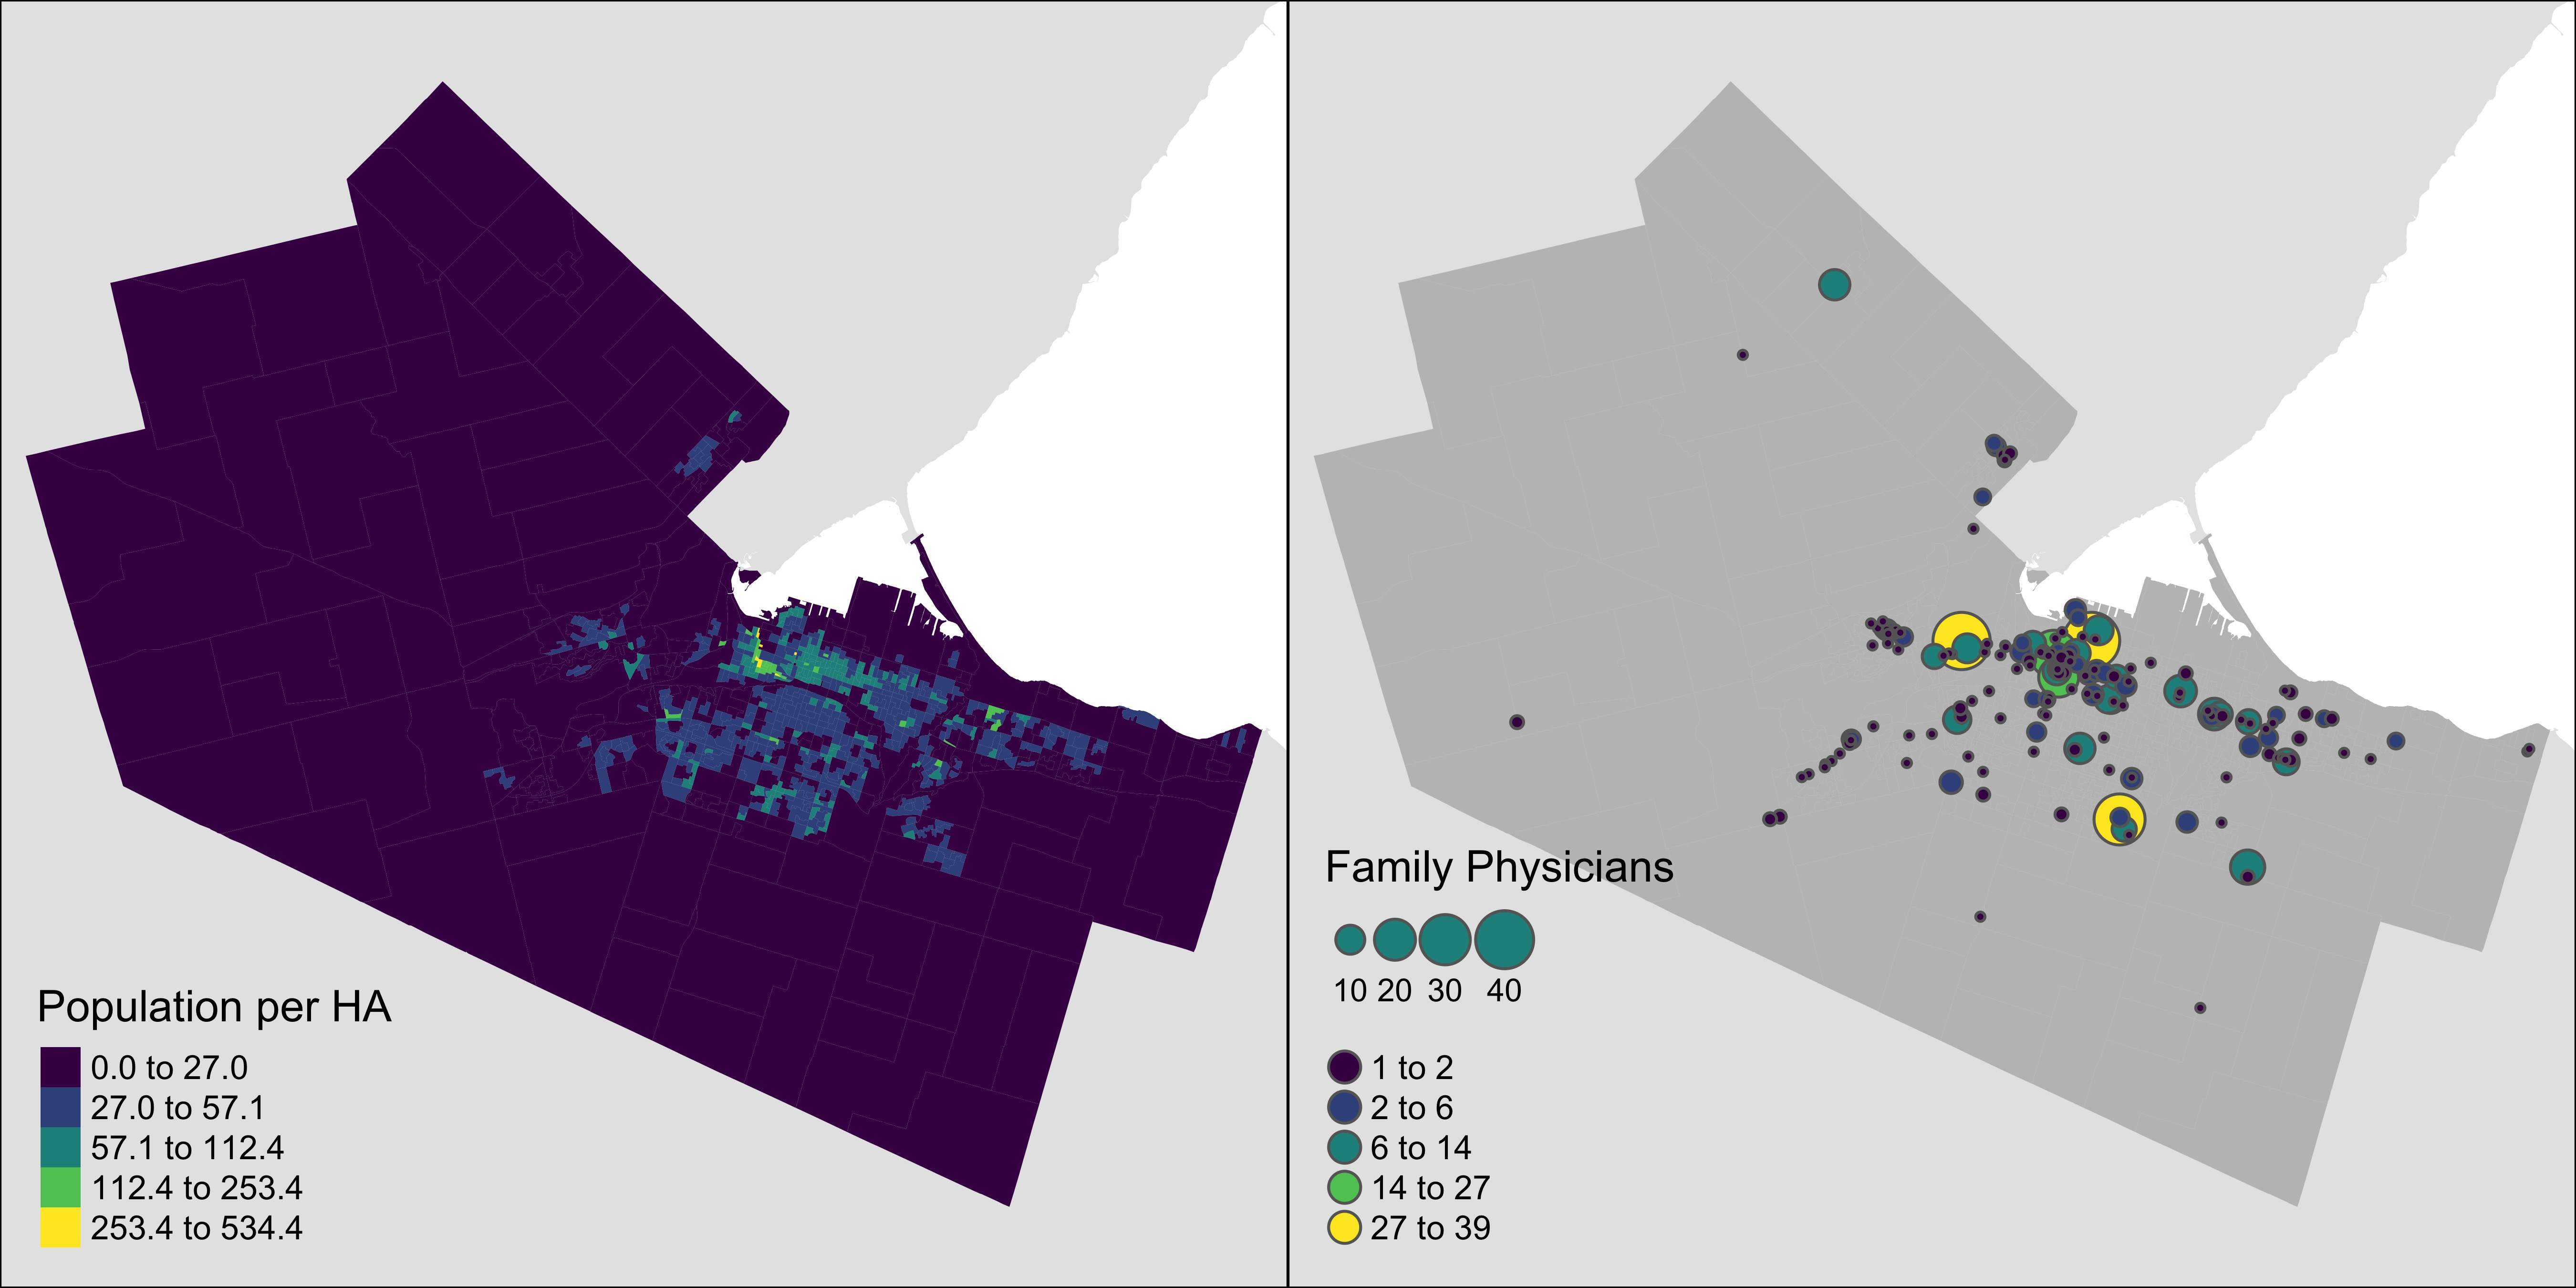
\includegraphics[width=1\linewidth]{./img/study_area_map} \caption{\label{fig:study_area_map}Population Density and Physician Locations}\label{fig:plot study_area_map}
\end{figure}

\hypertarget{results}{%
\section{Results}\label{results}}

\hypertarget{demand-and-clinic-level-of-service}{%
\subsection{Demand and Clinic Level of
Service}\label{demand-and-clinic-level-of-service}}

To compare the three methods, we focus first on the results associated
with how each of the methods calculates demand and levels of service at
the clinic locations. The level of service for the FCA approaches is the
local provider-to-population ratio (PPR) for each clinic while the MNL
model calculates trip demand-to-patient capacity ratios (DCR). To make
this comparable, we first take the inverse of the MNL ratios to reflect
patient capacity-to-trip demand ratio (CDR). Figure \ref{fig:ppr_dist}
displays a pair plot of the density of each level-of-service statistic
and their relationship and correlations with one another. The plot
highlights how the 2SFCA and B2SFCA methods are fundamentally similar in
the ways in which they allocate demand to the clinics with only a few
clinics above or below the scatterplot trend line. Likewise, it is
interesting to note the relatively high correlations between the PPRs at
the clinics in the FCA methods and the capacity-to-demand ratios in the
MNL model with the scatterplot revealing some non-linearity in this
relationship across the methods.

\begin{figure}
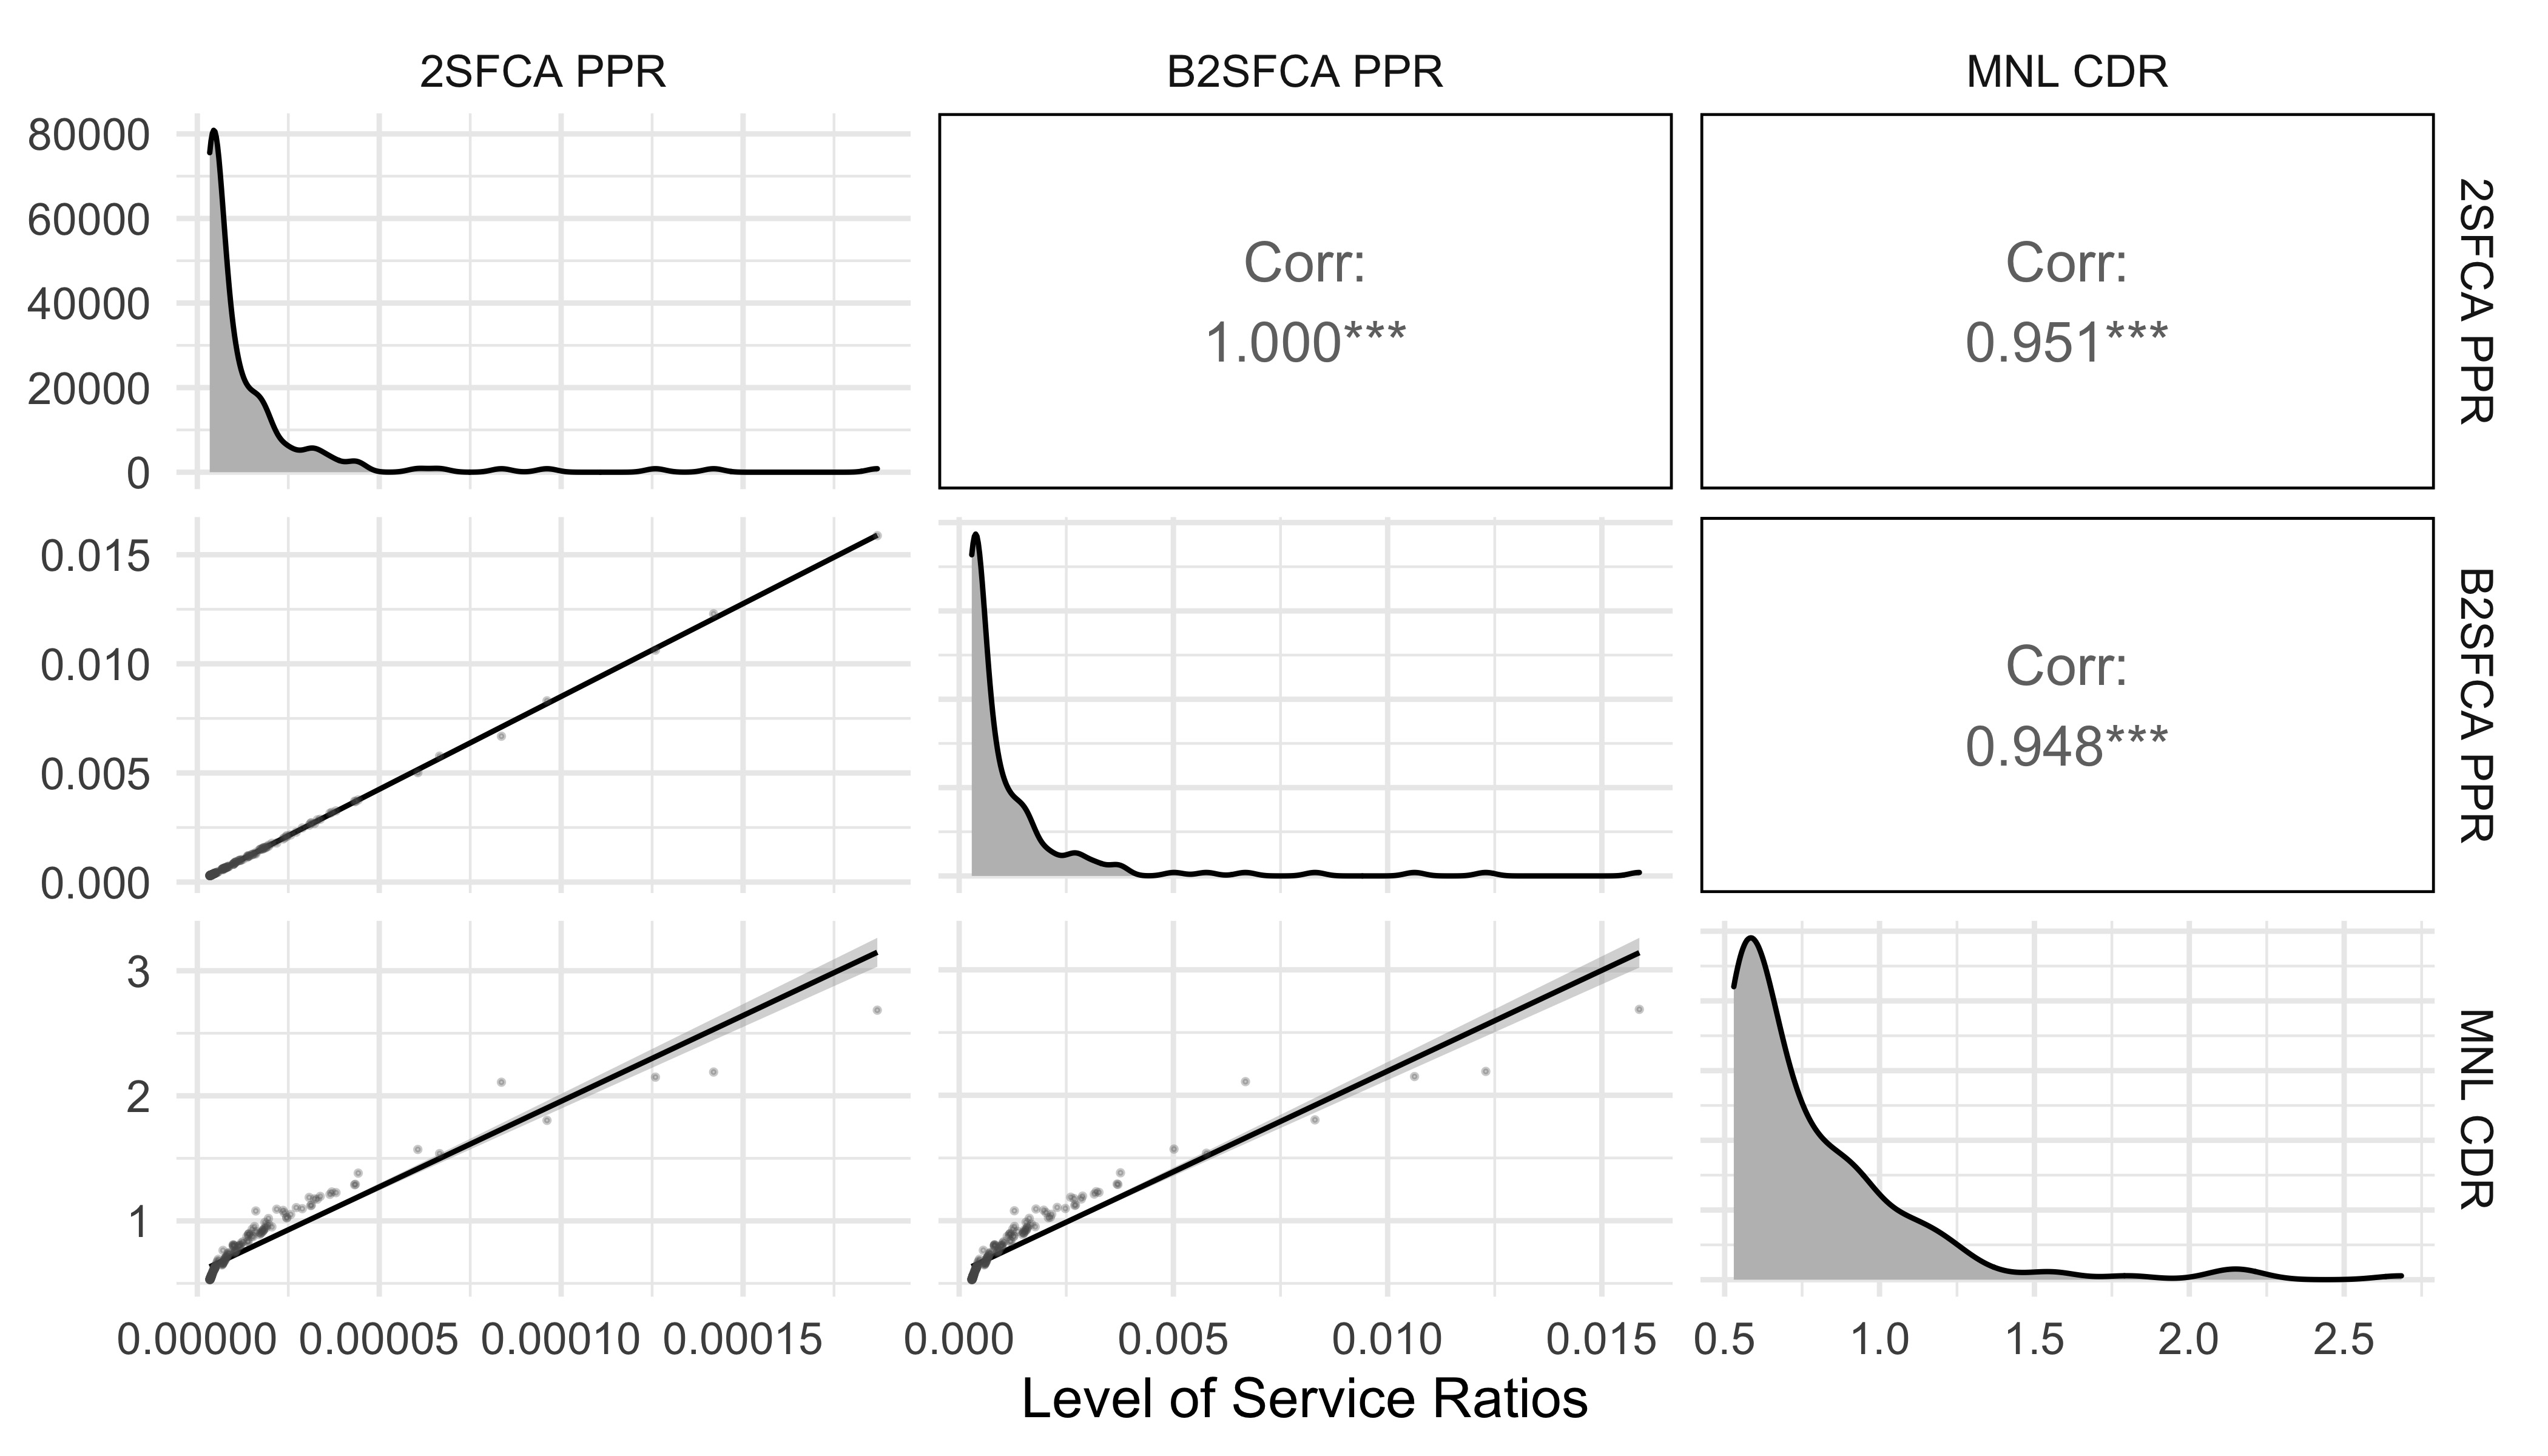
\includegraphics[width=1\linewidth]{./img/pair_plot_ppr} \caption{\label{fig:ppr_dist}Comparing Level of Service Distributions}\label{fig:ppr_dist_fig}
\end{figure}

Figure \ref{fig:los_maps} displays the levels of service for the clinic
locations. In general, more urban clinics tend to exhibit higher levels
of demand and lower levels of service across all three models. However,
the PPR values for the individual clinics in the 2SFCA are extremely
small compared to results from the B2SFCA model, highlighting how the
original method's multiple counting tends to inflate the (travel time
weighted) population numbers in each clinic's catchment and deflate the
level of service available at the clinics. In contrast, the PPRs in the
B2SFCA method are readily interpretable as the local ratio of doctors
per person for a given clinic considering the (travel-time weighted and
apportioned) populations within its catchment. Similarly, the MNL CDRs
reflect the relationship between the trip demand and patient capacity
based on the assumed rates. In terms of spatial trends, results from the
2SFCA and MNL models suggest both calculate higher levels of service at
larger clinics in the urban core as well as at a larger clinic in the
city's rural north-west. In contrast, the B2SFCA method generally
produces higher levels of service in an east-to-west direction. This
could reflect boundary effects in the study area that omit the large
populations present in the rest of the Greater Toronto Area on the
northern side of Lake Ontario that may also have access to these clinics
by driving.

\begin{figure}
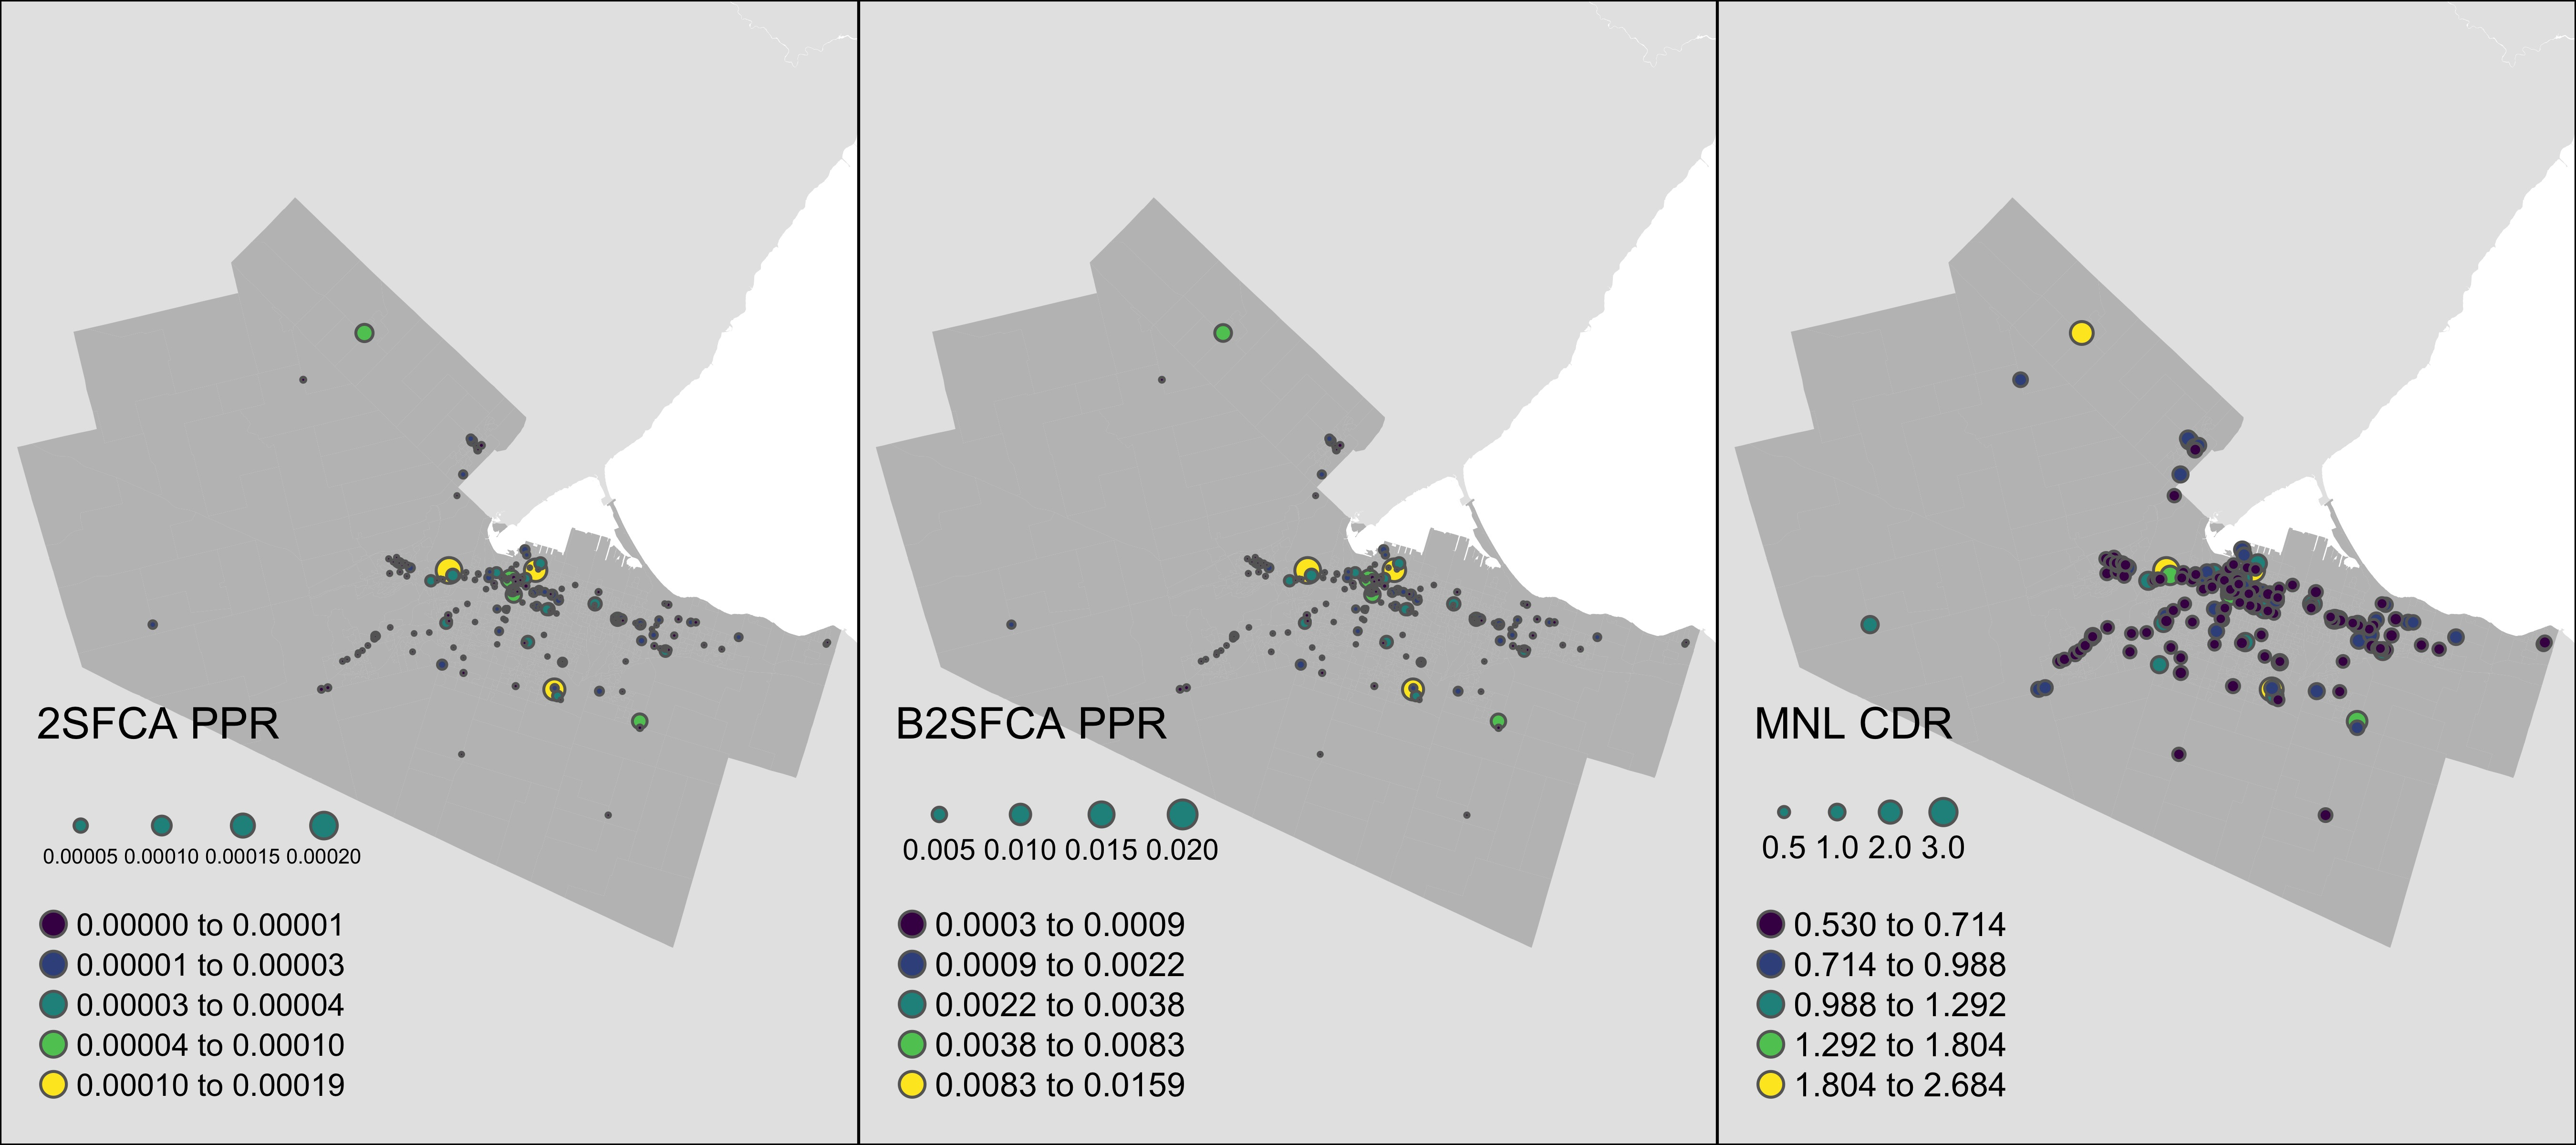
\includegraphics[width=1\linewidth]{./img/los_maps} \caption{\label{fig:los_maps}Calculated Clinic Levels of Service}\label{fig:los_maps_fig}
\end{figure}

\hypertarget{healthcare-accessibility}{%
\subsection{Healthcare Accessibility}\label{healthcare-accessibility}}

With the levels of service calculated above, the three models then
calculate accessibility to healthcare services in Hamilton.
Distributions, relationships, and correlations for the accessibility
results are shown in Figure \ref{fig:access_dist}. In this case, all
three models are highly correlated. The 2SFCA and B2SFCA produce nearly
identical distributions of results, although in the case of the balanced
method, the accessibilities correspond to the sum of travel time
weighted and apportioned provider-to-population ratios available in the
population zones free of the inflation and deflation that occurs in the
2SFCA. In contrast, the scatterplots of the MNL results again highlight
some non-linearity in the way the utility-based accessibilities are
calculated compared to the FCA methods. The thinner tail of the MNL
distribution suggests the method also results in fewer population zones
with lower accessibility compared to the FCA methods.

\begin{figure}
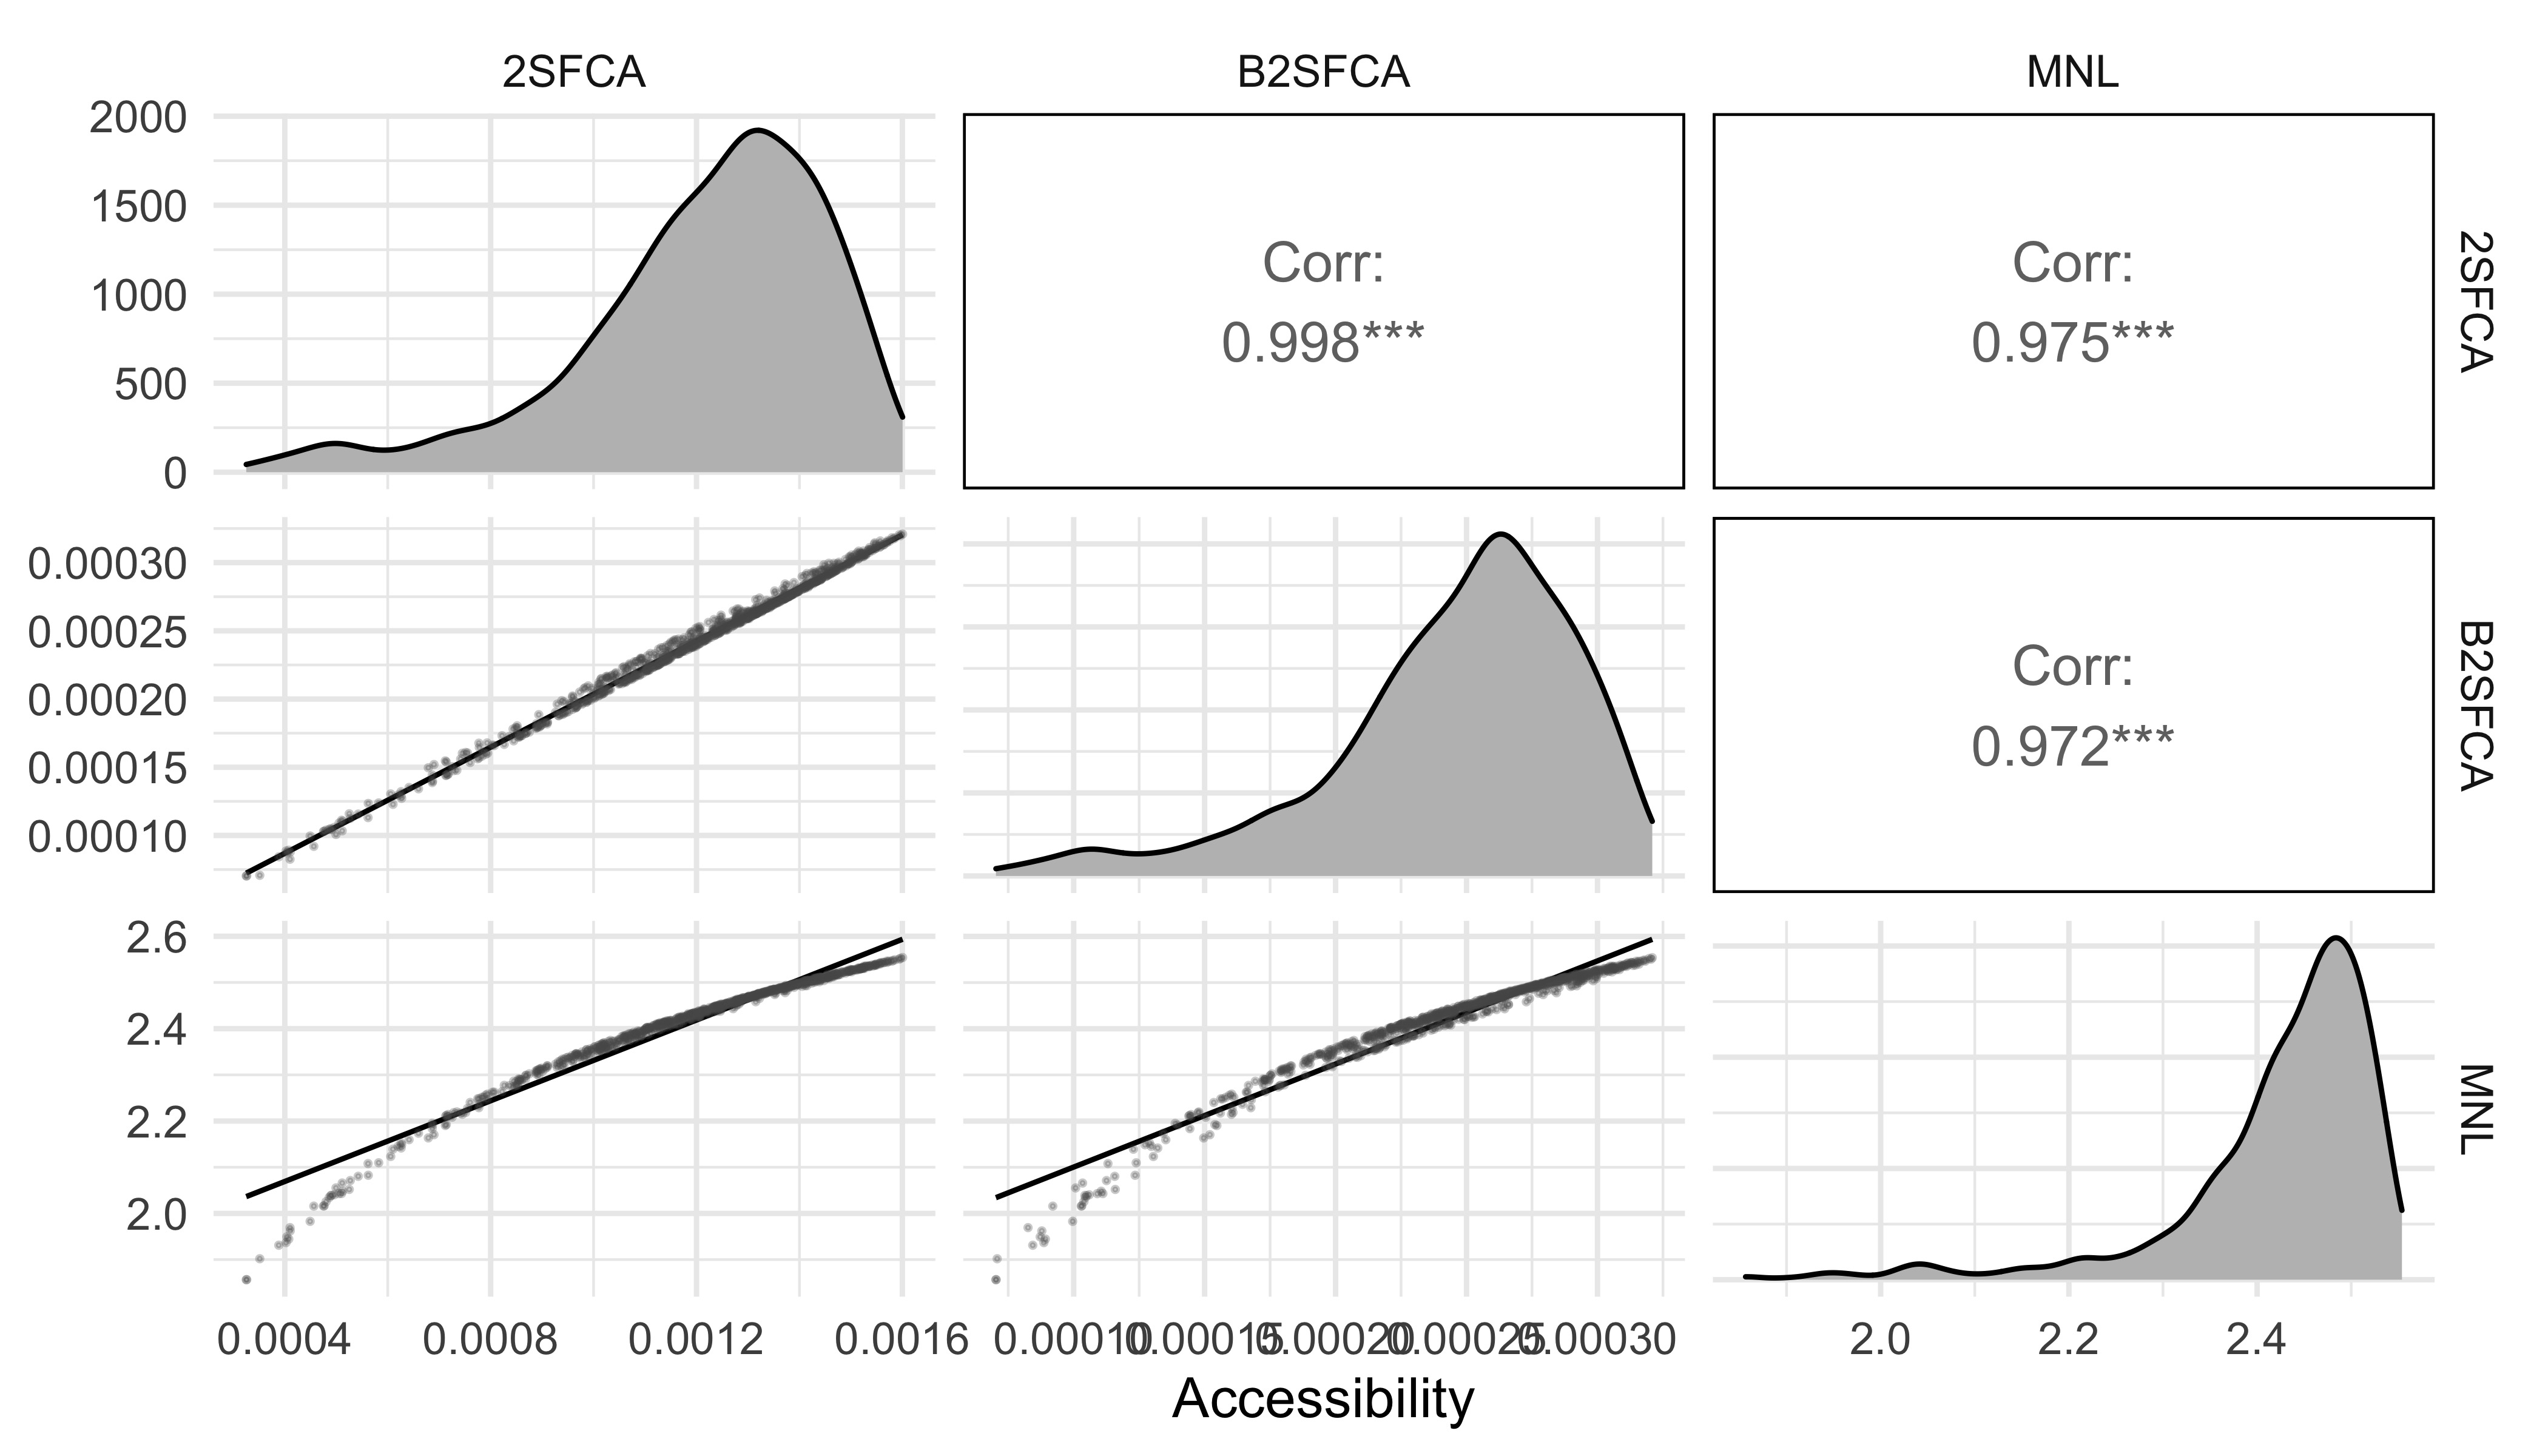
\includegraphics[width=1\linewidth]{./img/pair_plot_access} \caption{\label{fig:access_dist}Comparing Accessibility Distributions}\label{fig:access_dist_fig}
\end{figure}

The general spatial trends are similar across all three models (Figure
\ref{fig:access_maps}). The absolute accessibility values differ in
accordance with the ways each method calculates its accessibility
results. The FCA methods define accessibility based on the
physician-to-population ratios of clinics, resulting in smaller values.
In contrast, the MNL method defines accessibilities as the logsum of the
multinomial logit model, resulting in larger values that have no direct
interpretation. In general, the highest accessibilities to primary care
physicians correspond to the downtown area of Hamilton, where a large
number of clinics are concentrated. Accessibility to physicians
generally decreases with increased distance from the downtown area.

\begin{figure}
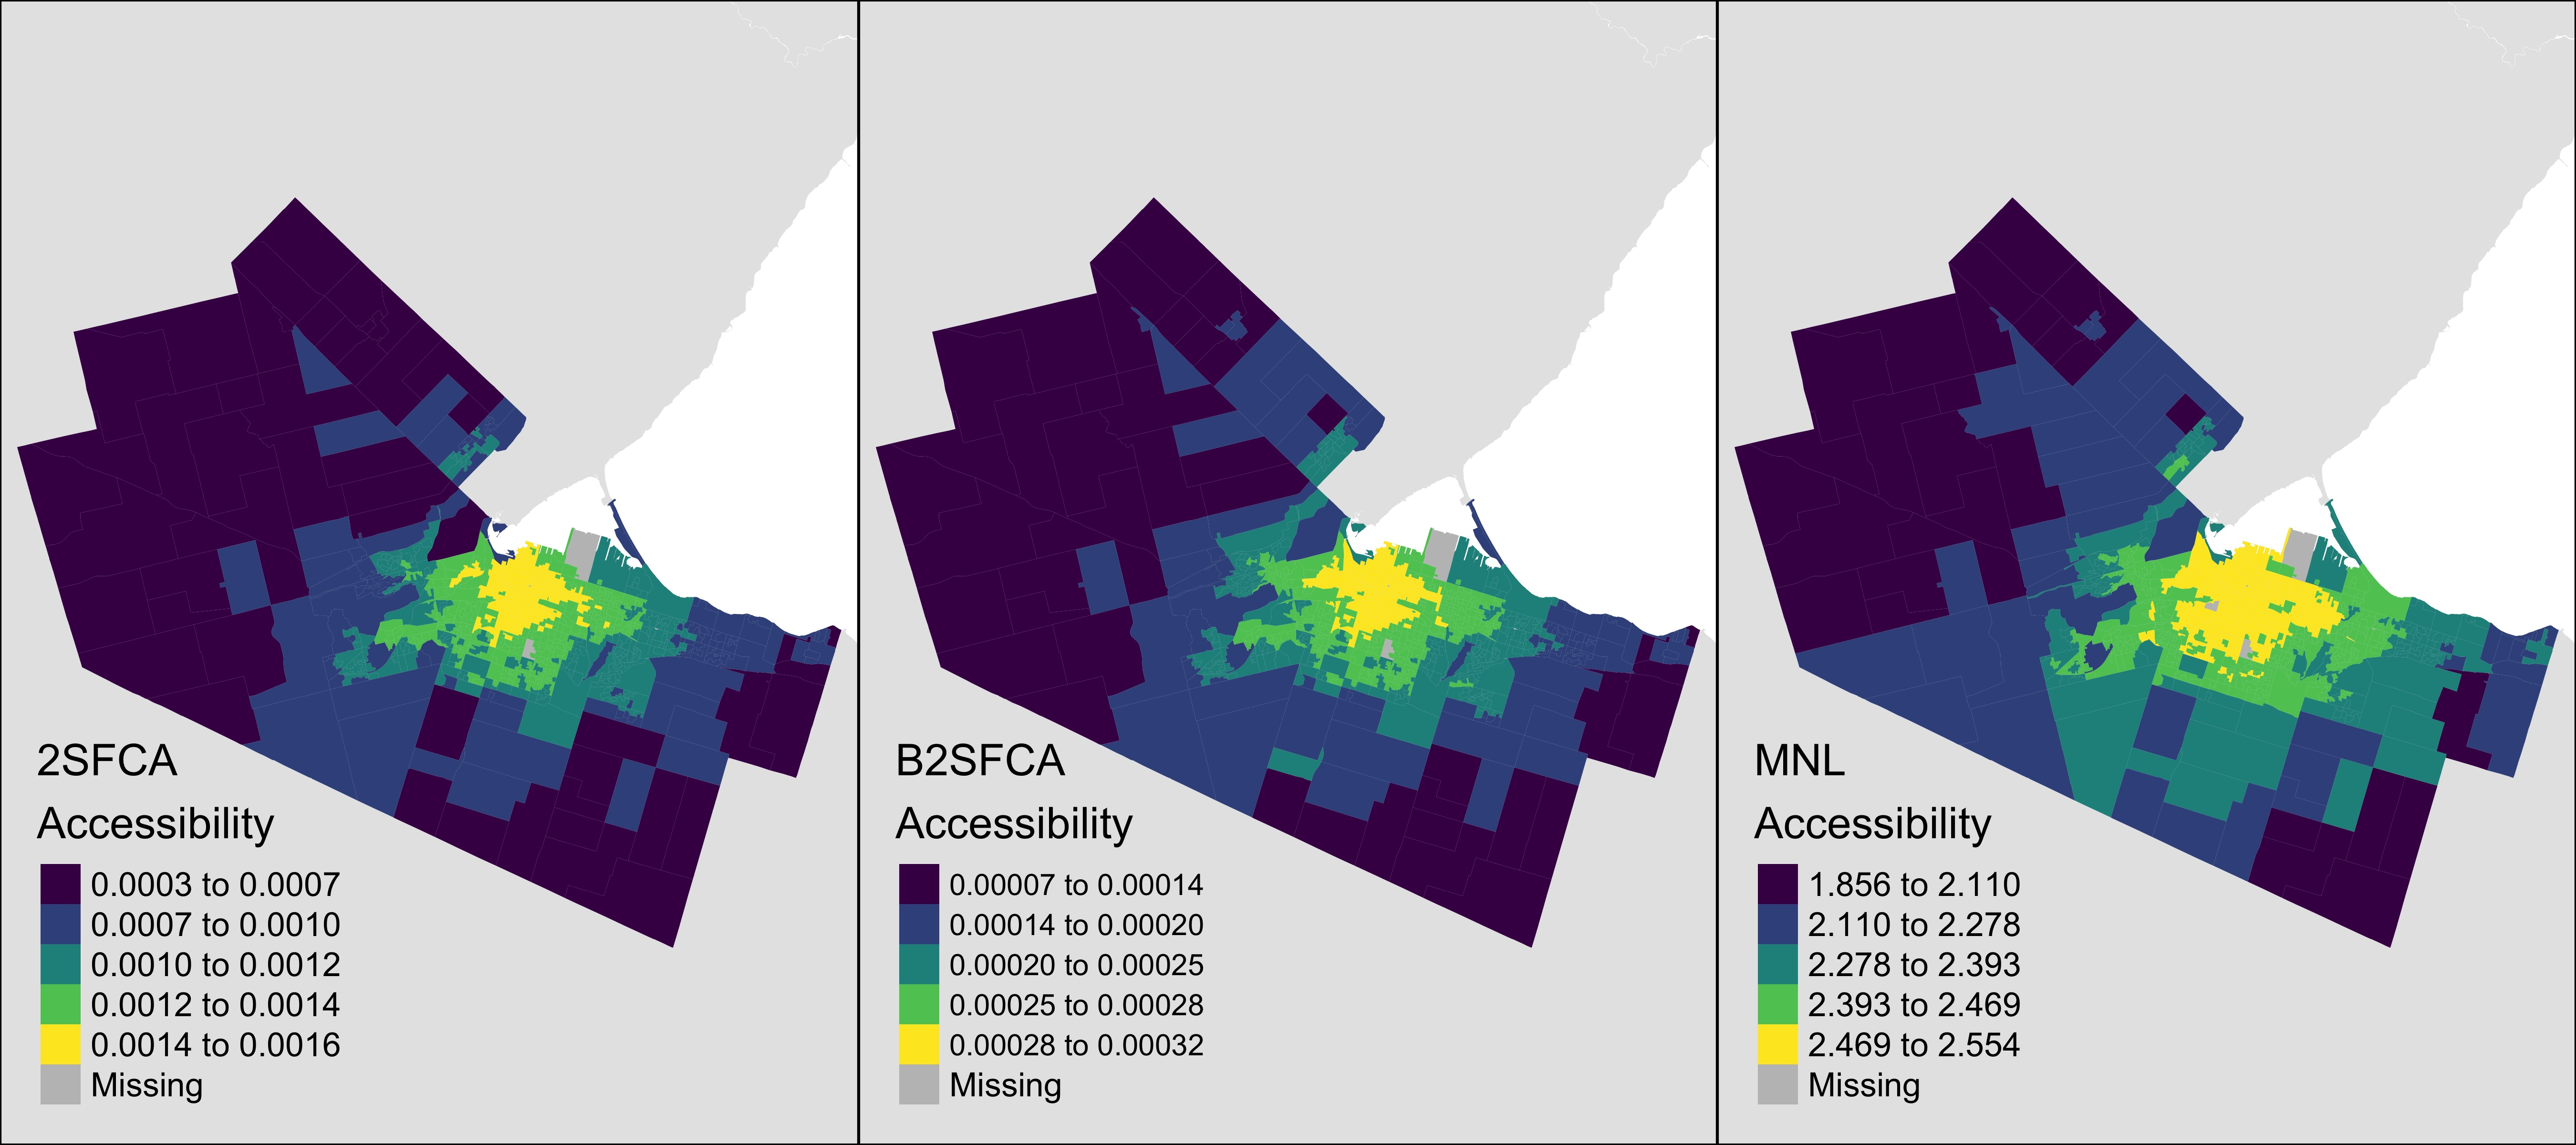
\includegraphics[width=1\linewidth]{./img/access_maps} \caption{\label{fig:access_maps}Accessibility Results}\label{fig:plot access_maps}
\end{figure}

To better highlight significant differences in the spatial patterns of
accessibility produced by each method, Figure \ref{fig:access_diff_maps}
displays the absolute differences in the normalized accessibilities
across models. To make the values comparable, we first normalize each
accessibility vector between 0-1 and take the differences of the
normalized values across each approach. In general, the MNL method tends
to produce higher accessibilities for most zones compared to the FCA
methods. In line with the distributions above, the 2SFCA and B2SFCA
models appear to be most similar, with only slight absolute differences
in the calculated accessibility values.

\begin{figure}
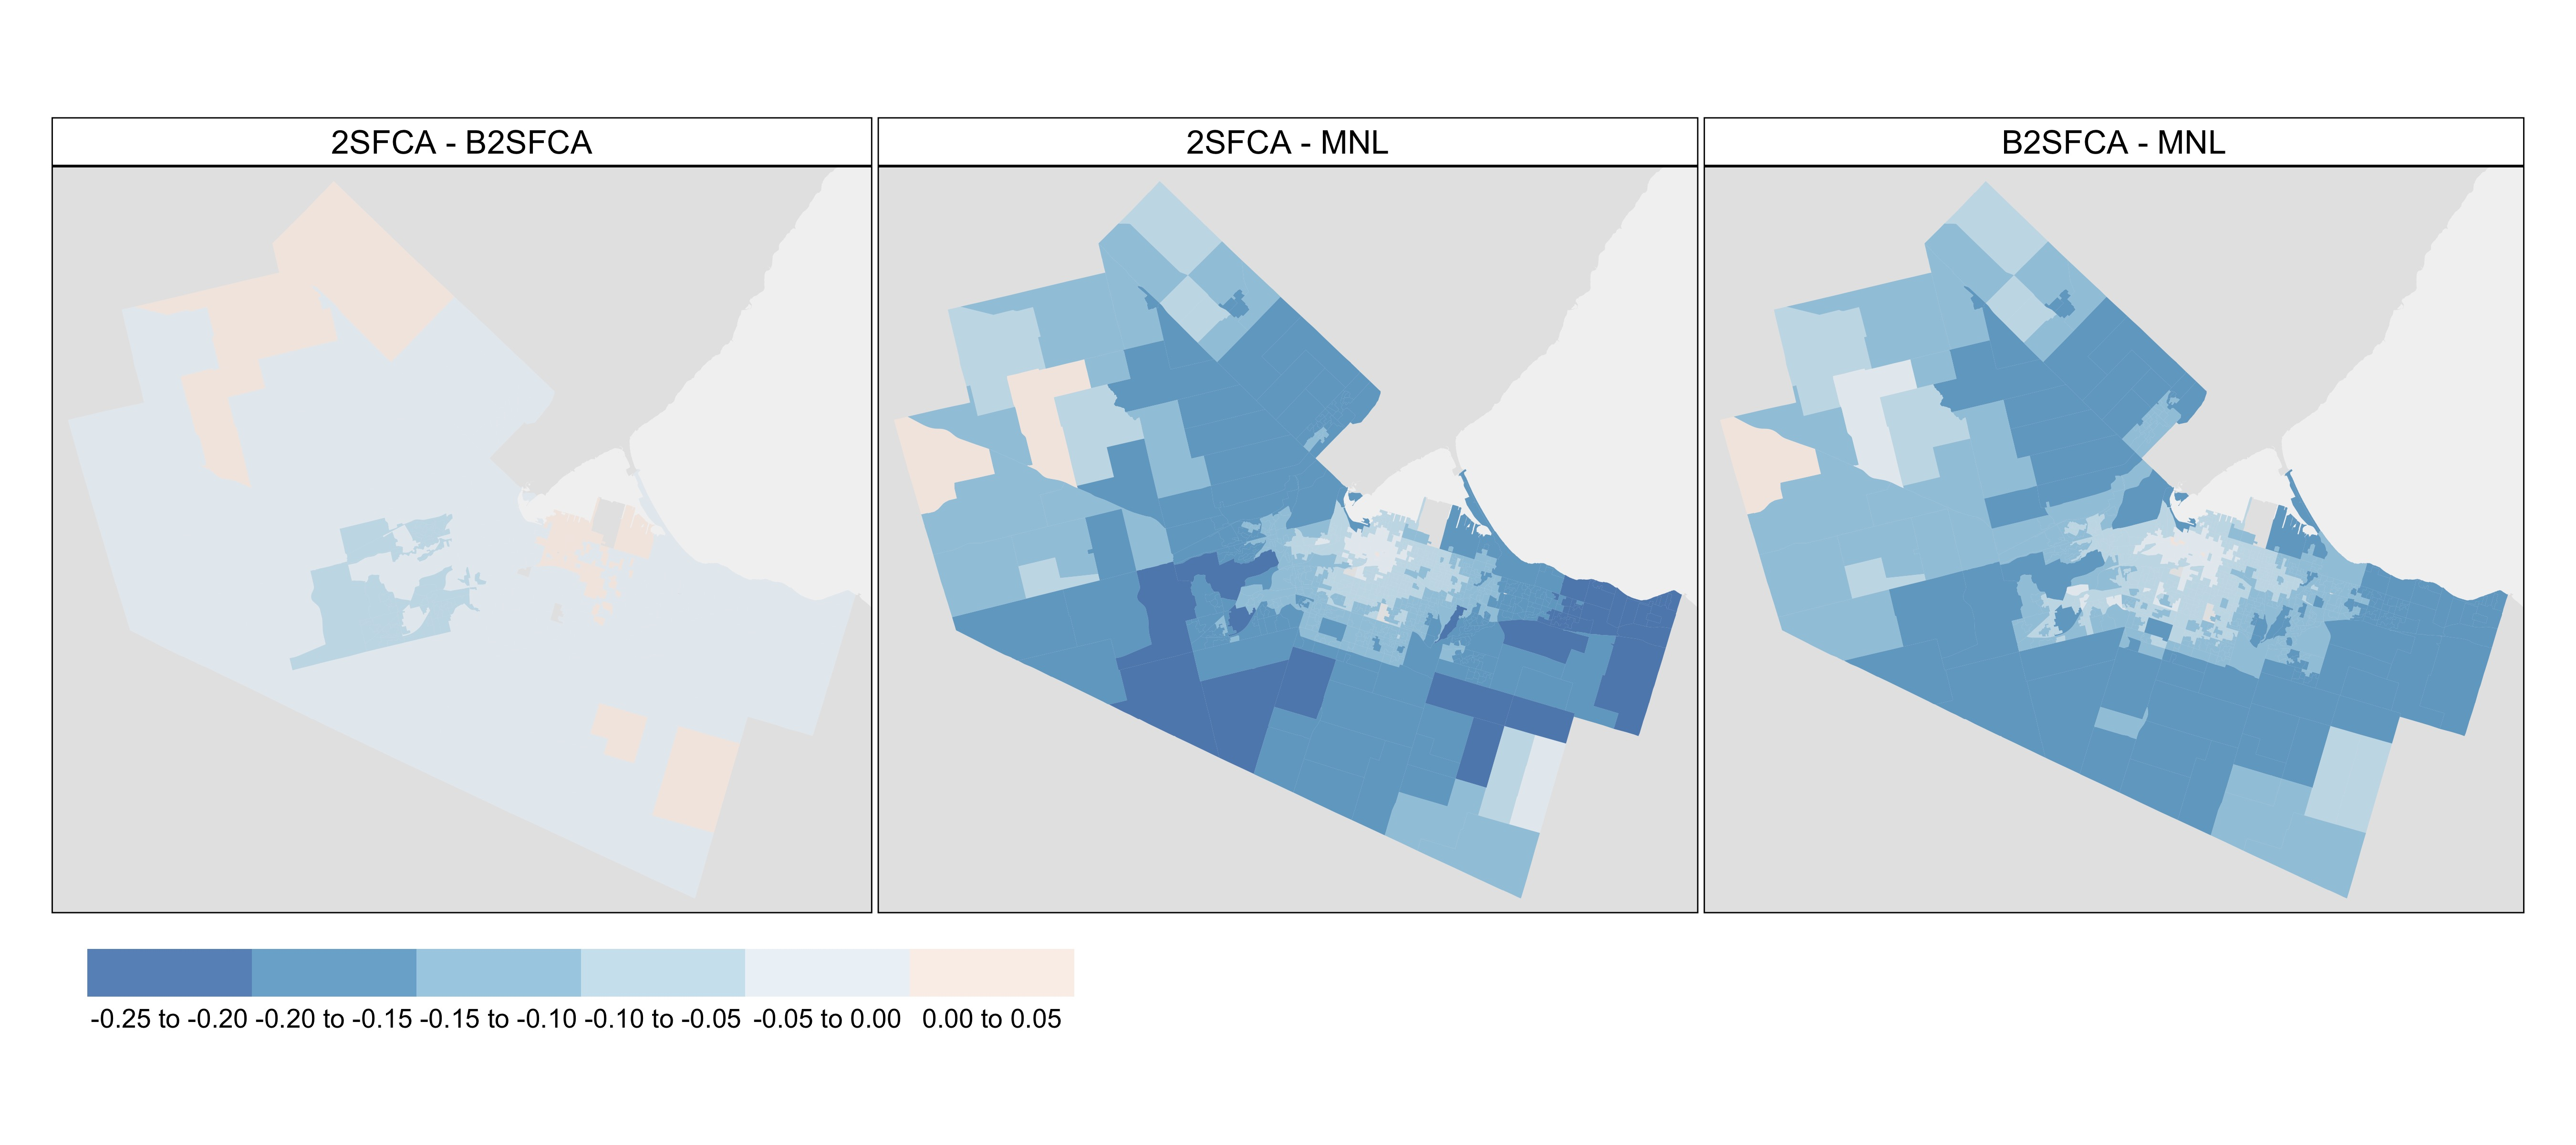
\includegraphics[width=1\linewidth]{./img/access_diff_maps} \caption{\label{fig:access_diff_maps}Normalized Accessibility Differences}\label{fig:plot access_diff_maps}
\end{figure}

To examine whether there are any spatial patterns in these differences,
Figure \ref{fig:access_locm_maps} plots the results of Local Moran's I
tests. The Local Moran's I is calculated on the differences using
queen-style contiguity weights, a critical significance level of
\(p=0.05\), and without correcting for multiple testing. The resulting
maps reveal some interesting patterns of spatial clustering in the
calculated normalized differences, particularly across the two FCA
models compared to the MNL model. Here, differences in accessibility are
greatest between the FCA and MNL methods in the low-low (LL) cluster in
the ring of outer suburbs that surround the city where the MNL model
tends to estimate higher accessibilities. In contrast, the calculated
accessibilities are more consistent across the methods in the high-high
(HH) cluster in the central part of the city. Differences in the
remaining zones are generally not significant (NS) aside from a very
small number of high-low (HL) and low-high (LH) outliers.

This overall pattern is likely due to the way the MNL approach handles
clinic choices with populations tending to select their nearest clinics.
On the one hand, the greater accessibilities in more suburban and rural
zones is likely derived from these populations accessing their closest
facility. On the other hand, this also means that fewer individuals from
more urban locations are competing for healthcare resources in these
more suburban and rural areas, leading to higher levels of service at
these suburban and rural clinics. In contrast, the FCA methods allocate
populations to all clinics within their catchment area using weights
derived from the impedance function. While this produces a smoothing of
the accessibilities, it can result in lower levels of service and
accessibility for clinics that populations may not actually use. This
effect seems to be minimized in more urban locations featuring higher
population densities and a greater number of clinics with available
physicians. Comparing the normalized results from the 2SFCA and the
B2SFCA models, the patterns of spatial clustering in the differences
appears to be less associated with the city's urban-suburban-rural urban
structure. While the B2SFCA method generally calculates slightly higher
accessibilities across the western half of the city, the methods are
most dissimilar in the south-east rural area.

\begin{figure}
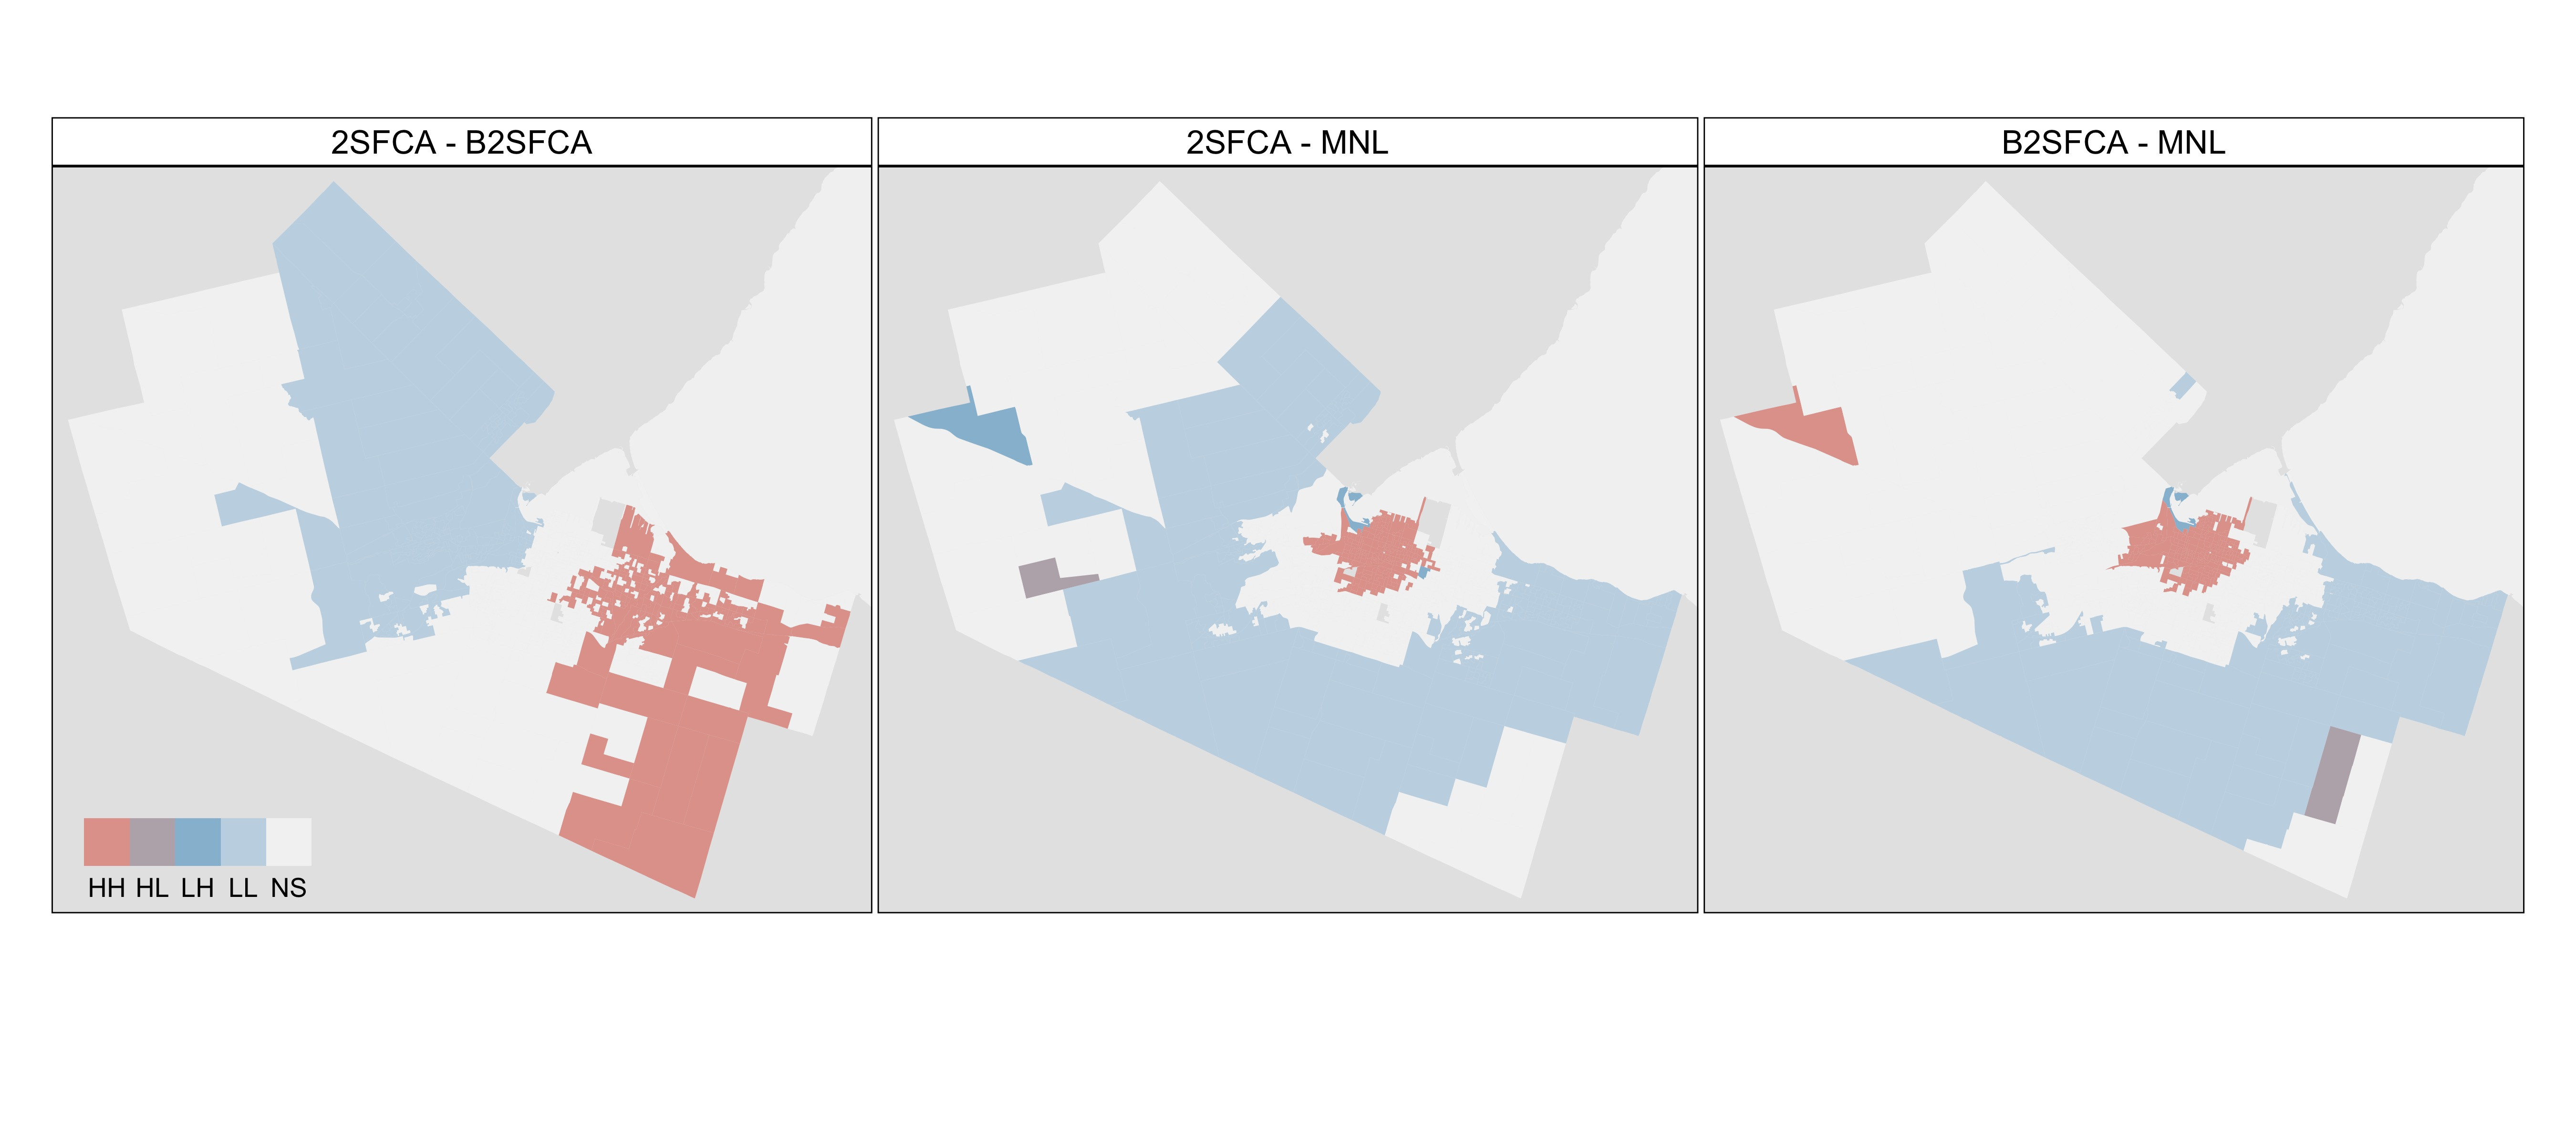
\includegraphics[width=1\linewidth]{./img/access_locm_maps} \caption{\label{fig:access_locm_maps}Accessibility Difference Hot Spots}\label{fig:fig 4}
\end{figure}

\hypertarget{sensitivity-analysis}{%
\section{Sensitivity Analysis}\label{sensitivity-analysis}}

In order to assess the impact of the \(\beta_{K+2}\) and
\(\beta_{K + 3}\) parameters on the results generated by the MNL method,
a sensitivity analysis was undertaken. The \(\beta_{K+2}\) parameter
that influences the attractiveness of higher-capacity clinics was
gradually increased from 0.1 to 1 and the \(\beta_{K + 3}\) parameter
that influences sensitivity to congestion or crowding at the clinics was
gradually increased from -1 to -0.1. Increments of 0.1 are used for each
variable. Results are summarized by calculating average CDRs and
accessibilities across the clinics and DAs respectively in each of the
100 scenarios (Figure \ref{fig:sensitivity_plot}). Two example scenarios
are also created for illustration. In Scenario 1, the \(\beta_{K+2}\)
parameter was decreased from 1 to 0.5 relative to the original
calculations while the \(\beta_{K + 3}\) parameter was decreased from
-0.5 to -1 in Scenario 2.

For the CDRs in the left panel of Figure \ref{fig:sensitivity_plot}, the
sensitivity analysis reveals that decreasing sensitivity to the
attractiveness of capacity (as \(\beta_{K+2}\) approaches 0.1) and
decreasing sensitivity to overcrowding (as \(\beta_{K+3}\) approaches
-0.1) combine to produce more balance between the supply of physician
capacities and patient demand, on average. Examining the clinic data in
greater detail, this weighting results in more trips being made to
smaller and more congested clinics relative to larger ones where there
is more supply relative to demand. Greater weight placed on facility
capacity (as \(\beta_{K+2}\) approaches 1) and high sensitivity to
overcrowding (as \(\beta_{K+3}\) approaches -1) also results in more
balanced CDRs, but in this case, more trips are made to larger clinics
that become more congested versus smaller ones that are less congested.
Scenarios along the diagonal exhibit relatively less balance, on
average, across the clinics.

In terms of accessibilities, average accessibilities are, in general,
more sensitive to changes in the \(\beta_{K+2}\) parameter than
\(\beta_{K+3}\). Comparing the original results against Scenario 1,
average accessibilities increase by around 22\% when \(\beta_{K+2}\)
increases from 0.5 to 1. In contrast, access increases by about 11\%
across Scenario 2 and the original calculations as the \(\beta_{K+3}\)
sensitivity to overcrowding parameter decreases in weight from -1 to
-0.5. The greatest average accessibilities in \ref{fig:sensitivity_plot}
result from high attractiveness to clinic capacity and low weight on
overcrowding (\(\beta_{K+2} = 1\) and \(\beta_{K+3} = -0.1\)), leading
to more trips made to smaller overcrowded clinics that are more evenly
distributed around the city and likely closer to the origins in terms of
travel time relative to some of the larger clinics that are more
centrally-located.

To examine whether the sensitivity analysis impacts the spatial
distributions of calculated accessibilities, Figure
\ref{fig:sensitivity_maps} plots normalized accessibility results from
the original and two sensitivity scenarios. Although both adjustments to
the parameters result in decreased absolute accessibilities in Figure
\ref{fig:sensitivity_plot}, comparisons of the normalized values suggest
there are no distinct spatial trends associated with changes in
\(\beta_{K + 2}\) and \(\beta_{K + 3}\) across the sensitivity
scenarios.

\begin{figure}
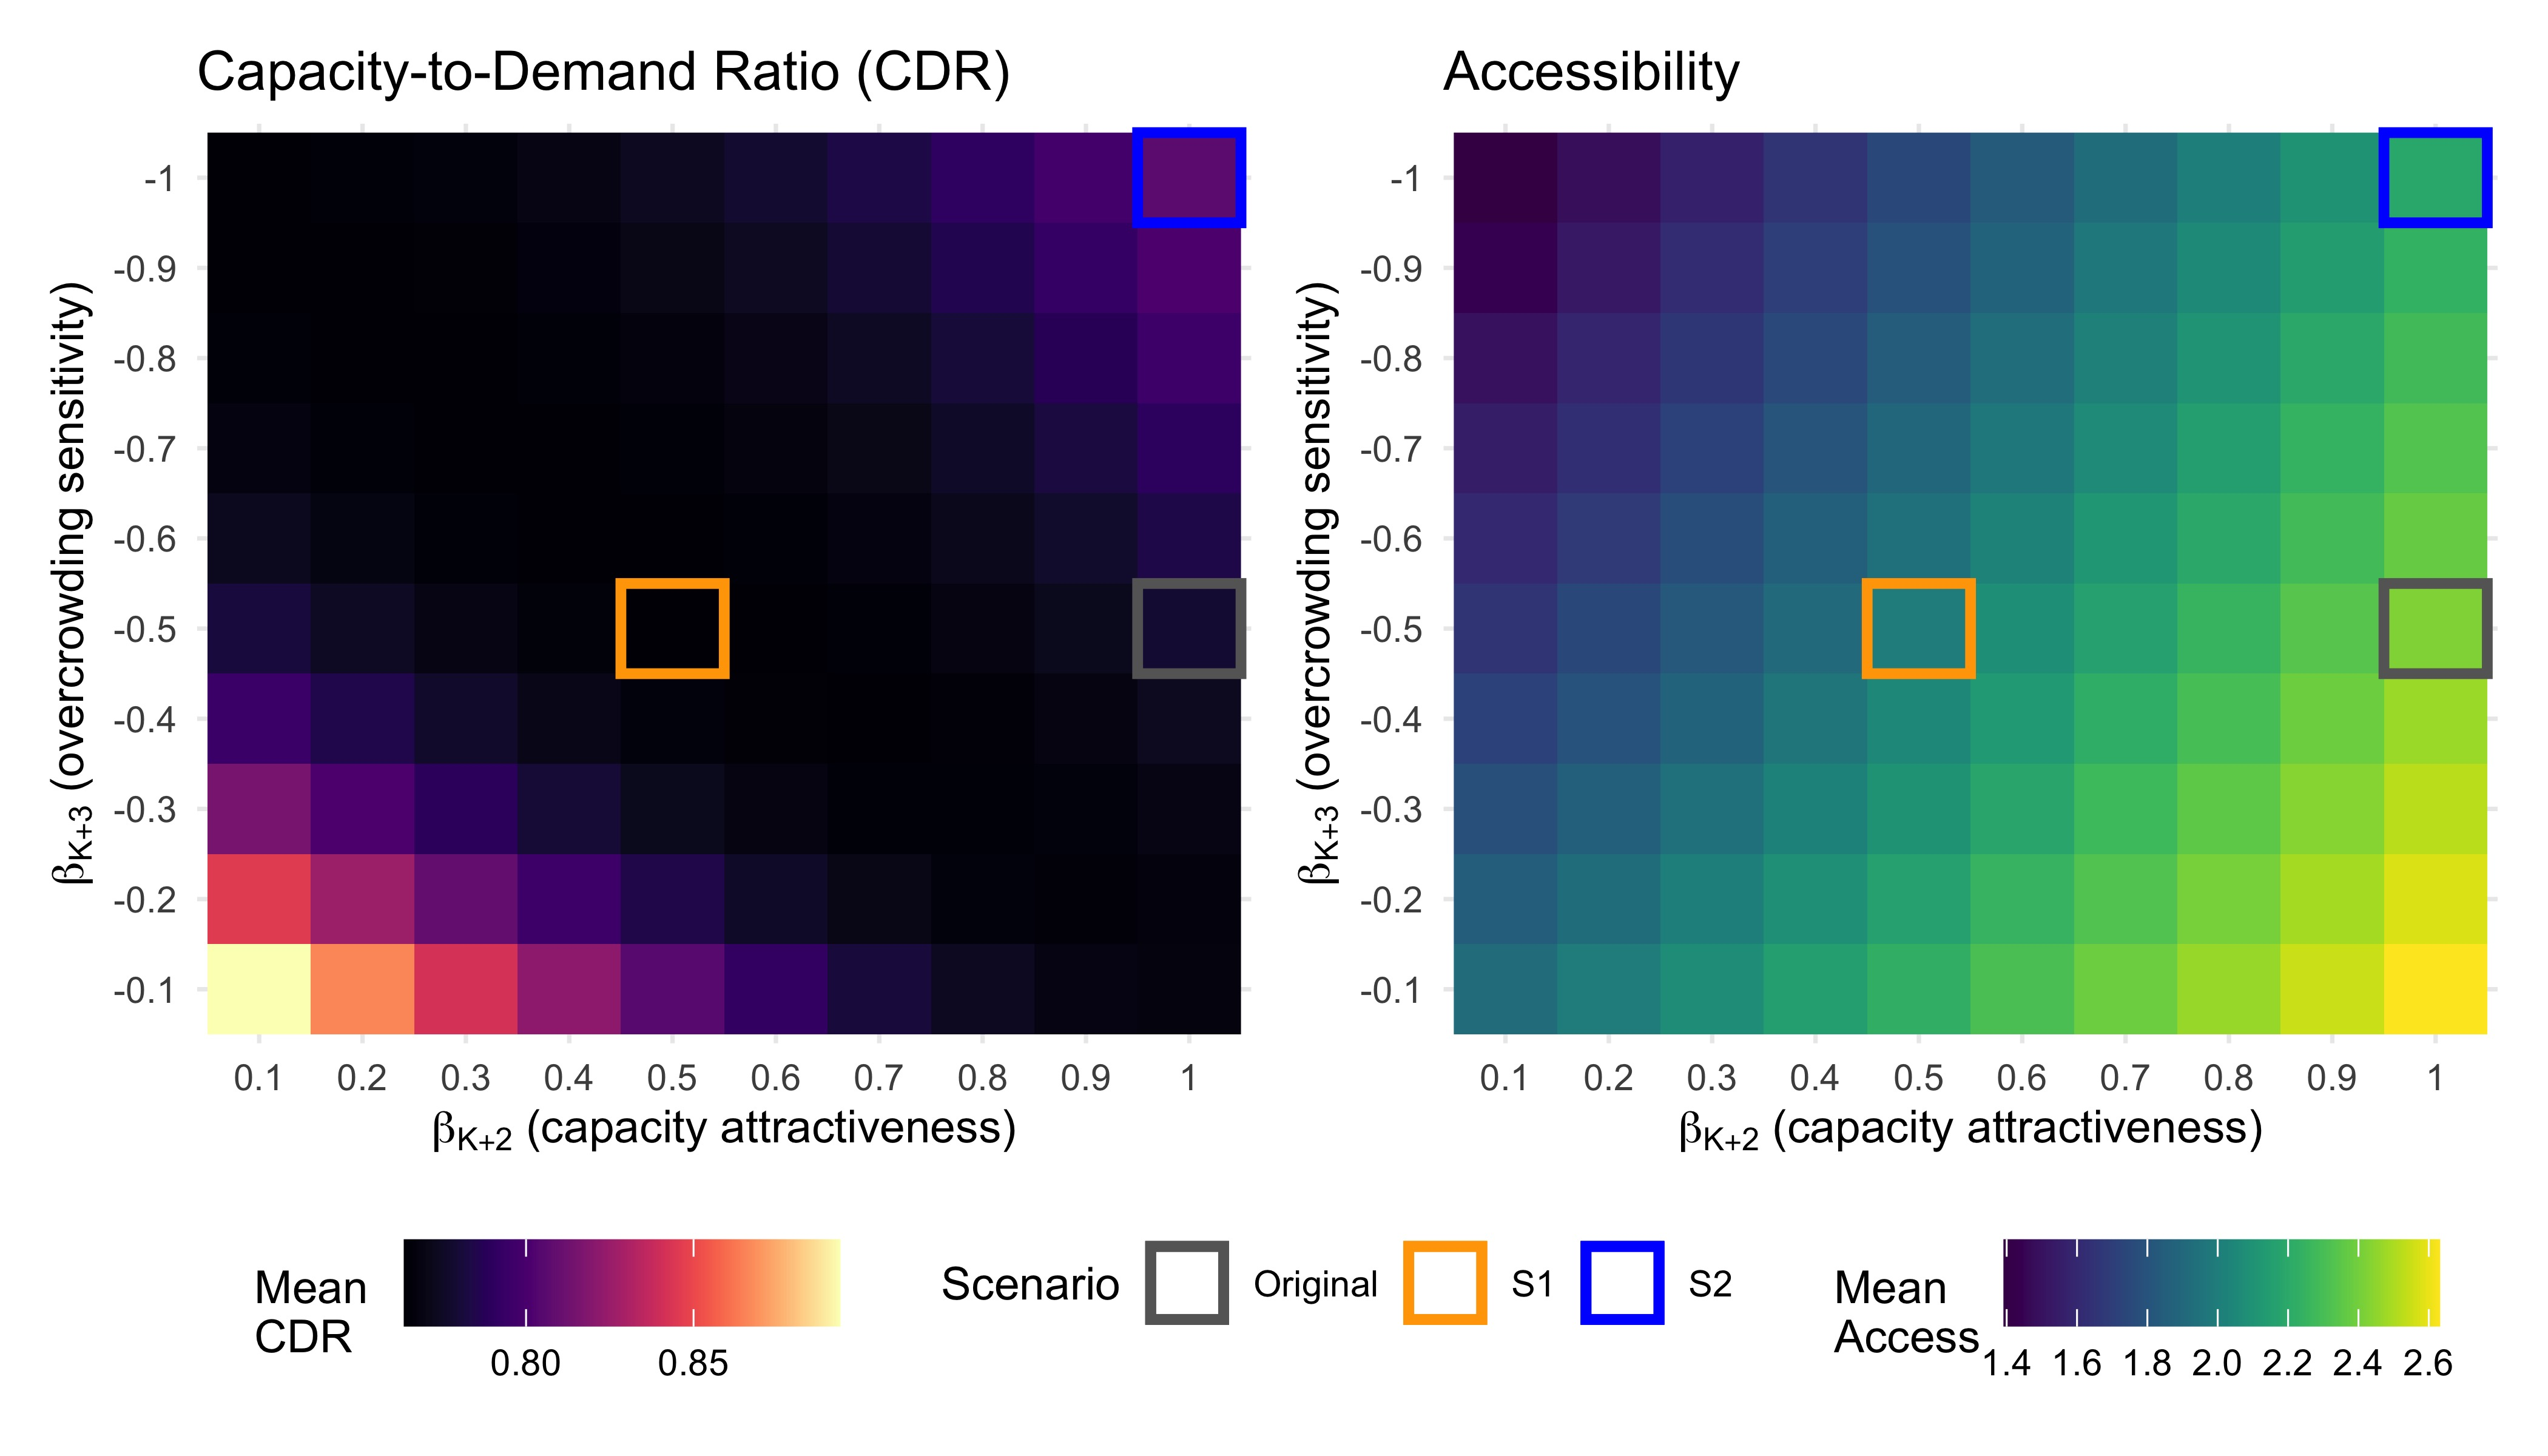
\includegraphics[width=1\linewidth]{./img/sensitivity_plot} \caption{\label{fig:sensitivity_plot}Sensitivity Analysis Results}\label{fig:plot sensitivity_tiles}
\end{figure}

\begin{figure}
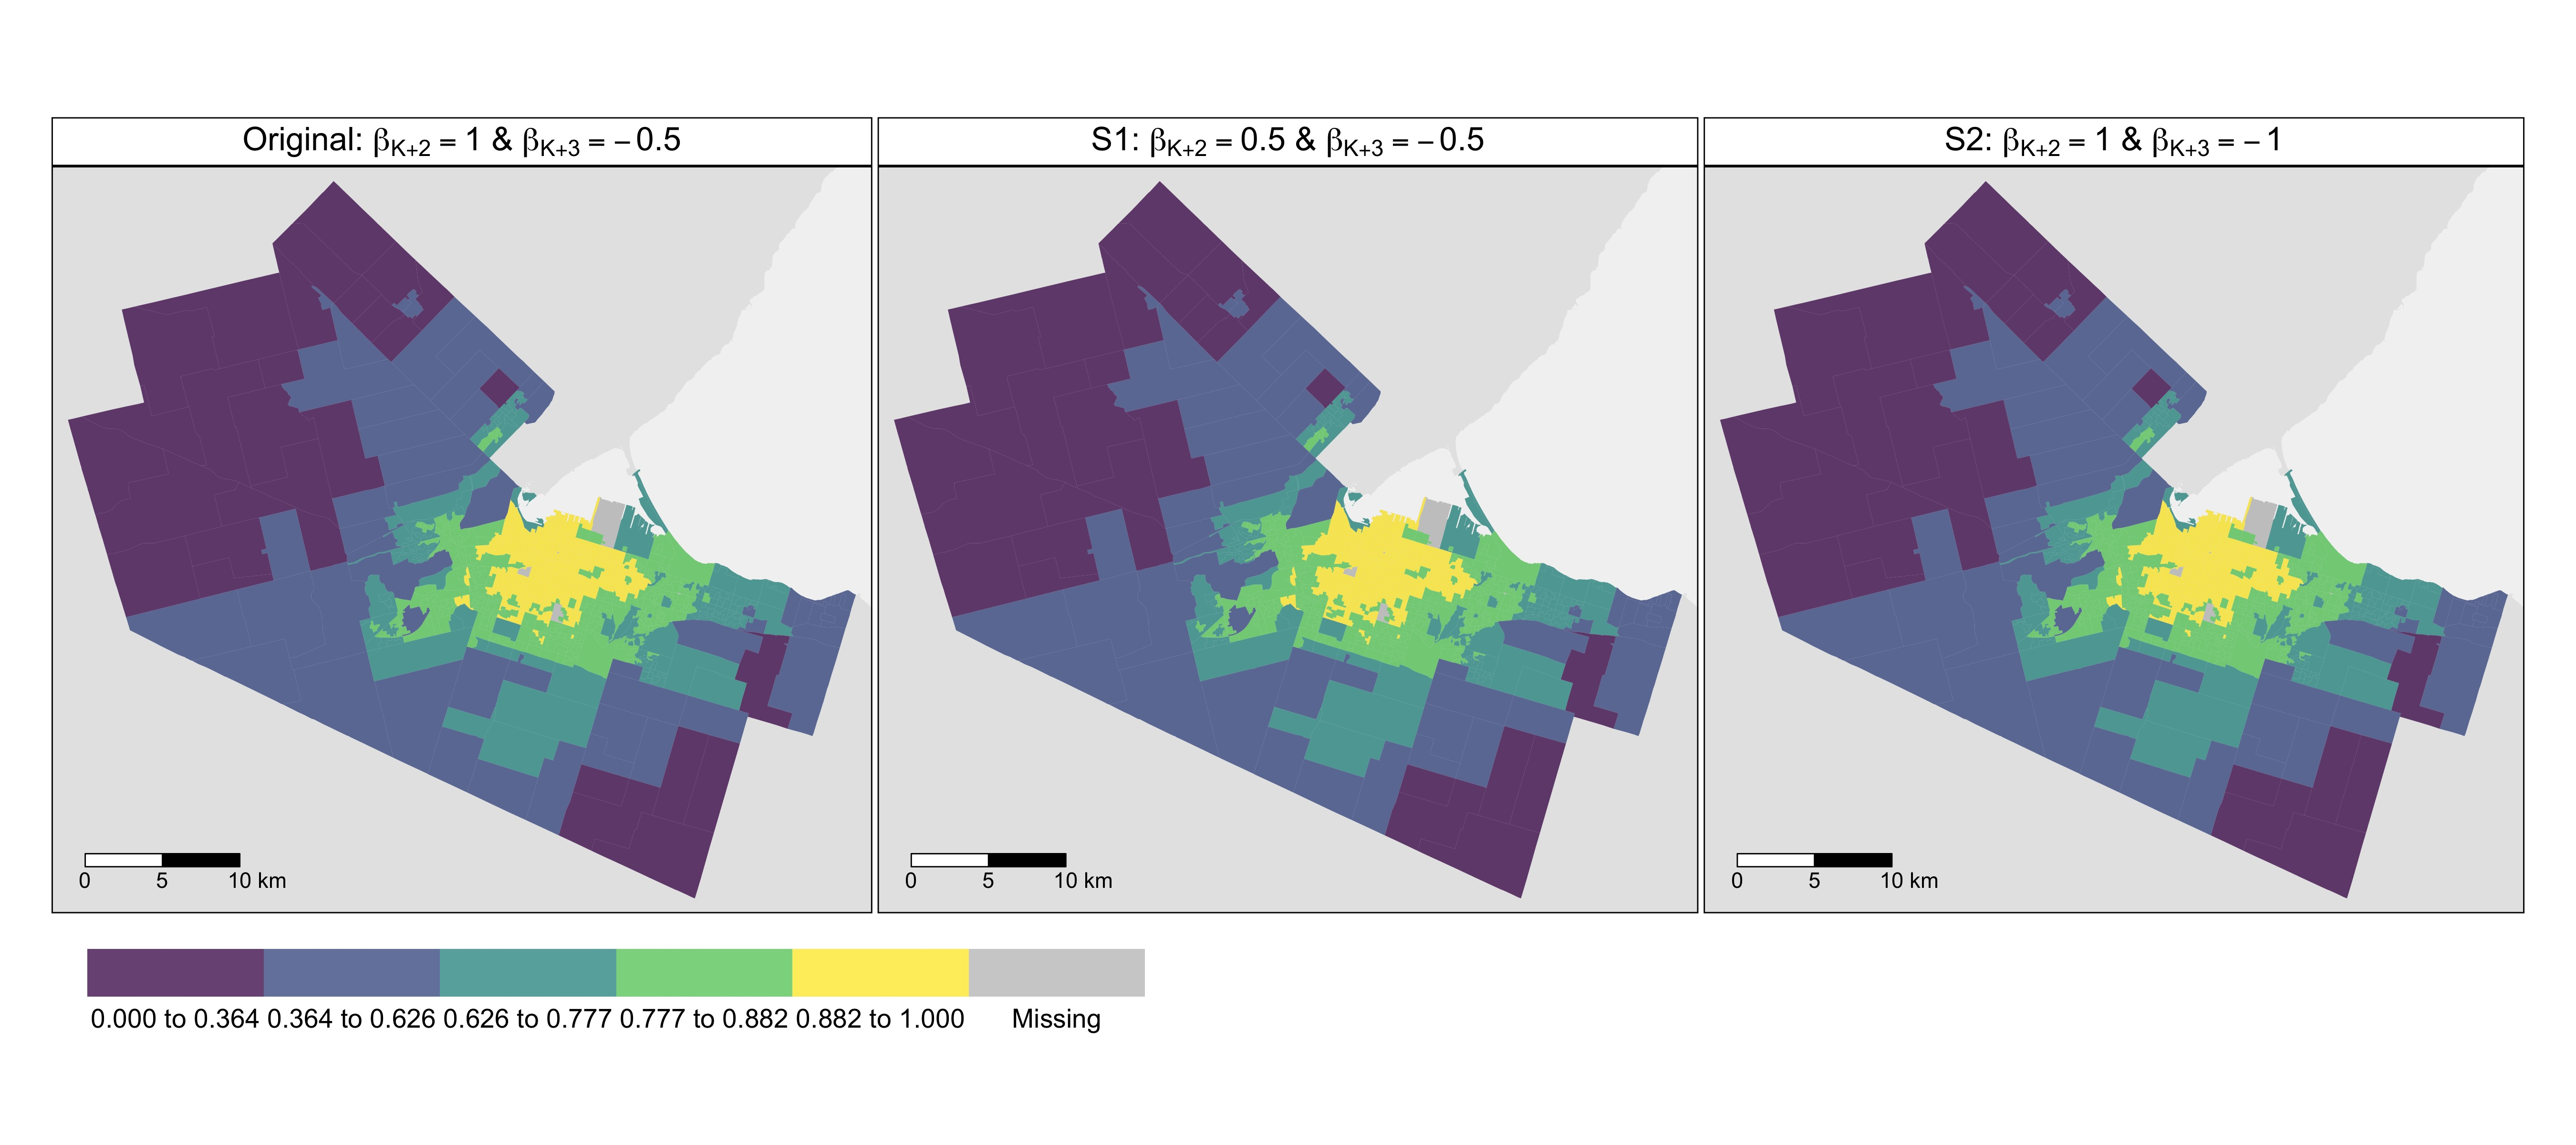
\includegraphics[width=1\linewidth]{./img/sensitivity_maps} \caption{\label{fig:sensitivity_maps}Sensitivity Scenario Maps}\label{fig:plot sensitivity_maps}
\end{figure}

As shown in the above figure, the accessibilities have decreased across
the City of Hamilton in both sensitivity analysis scenarios. However,
reducing the \(\beta_{K+2}\) parameter has a larger effect as compared
to reducing the \(\beta_{K + 3}\) parameter, with more dissemination
areas being in the lowest category of accessibilities. The model is
therefore more sensitive to the \(\beta_{K+2}\) parameter, however,
adjusting the \(\beta_{K + 3}\) parameter also has a large effect on the
results produced by the MNL method. It is therefore important to
calibrate the model's parameters in order to match observed trip
distributions in the City of Hamilton.

\hypertarget{discussion-and-conclusions}{%
\section{Discussion and Conclusions}\label{discussion-and-conclusions}}

Since the 2SFCA was proposed by Luo and Wang (2003), the floating
catchment area approach has been a popular one for calculating
place-based accessibility to healthcare services that considers both the
supply and demand components and several key innovations have been made
to FCA methods since. However, FCA methods are still limited in two
important ways. First, FCA methods do not fully consider aspects of
travel and choicemaking behaviour. Like many of the other place-based
accessibility measures, the only behavioural component of FCA methods is
the impedance function that is used to weight the value of opportunities
by the distance or travel time required to reach them. Second, FCA
approaches also tend to assign population demand and levels-of-service
to facilities or population zones in an overlapping manner, using the
impedance function (and other adjustments) to weight each value within a
catchment area. Crucially, this use of overlapping catchment areas in
previous FCA approaches has been shown to bias results by
inflating/deflating supply and demand. While the B2SFCA proposed by Páez
et al. (Paez et al., 2019) rectifies this, it does so by apportioning
fractions of populations and levels-of-service through adjustments to
the impedance function.

To respond to these issues, this research developed a multinomial logit
destination choice model for calculating utility-based transportation
accessibility to primary care physicians. While FCA approaches consider
accessibility in terms of provider-to-population ratios weighted by
distance or travel time, the MNL approach reframes the measurement of
health accessibility into individual trips to visit primary care
physicians and the utility-bearing aspects of clinics. With its basis in
random utility theory, the MNL model considers several additional
aspects that define the appeal of clinics in addition to the travel time
required to reach them, including the number of physicians available at
the clinic and the level of crowding. The destination choice model also
avoids multiple-counting as the iterative fitting procedure results in
the assignment of each patient trip to a single clinic on average.

Comparisons of the MNL approach with 2SFCA and B2SFCA models using data
for the City of Hamilton suggests that the accessibility patterns
produced by each method are broadly similar, with the highest
accessibilities in the central core of the city where many clinics and
physicians are located. However, further analysis of the distributions,
correlations, and spatial clustering of accessibility differences
reveals that the MNL method produces generally higher accessibilities
throughout much of Hamilton with the greatest differences seen in the
ring of suburban and rural zones that surround the city. It seems likely
that these results arise from the MNL model assigning trips based on the
most proximate clinic for these residents while more urban residents are
being drawn to more urban clinics. In contrast, the FCA approaches
assign population values to all clinics within their catchment area and
all population zones share the levels-of-service of accessible clinics,
likely leading to higher demand and lower available supply at these
rural and suburban clinics.

For planning and policy, our analysis suggests that both the B2SFCA and
MNL approaches offer merit. While the 2SFCA is generally straightforward
to calculate with limited data requirements, it has been shown to return
biased results as a consequence of double counting that makes the
interpretation of provider-to-population ratios and accessibility scores
problematic. The B2SFCA, on the other hand, requires the same data as
the 2SFCA method but improves on it by preserving the population being
serviced and the level of service. Both the levels-of-service and
accessibilities calculated in the B2SFCA method are readily
interpretable as population-to-provider ratios. However, the only travel
behaviour component in both the 2SFCA and B2SFCA approaches is the
impedance function. While it does tend to result in the greatest weight
placed on the nearest locations in practice, it still results in a
spreading or smoothing of demand and supply. In contrast, the MNL
model's utility-based approach has a stronger behavioral foundation and
considers more aspects that define the appeal of particular clinics. It
also appears to produce what are arguably more realistic results in
suburban and rural areas. However, the MNL approach is more data-hungry
and its results are highly sensitive to the parameter assumptions that
were made on the part of the research team. Moreover, the accessibility
scores have no direct healthcare interpretation.

All methods in our comparative study are limited due to the imposition
of boundary effects that likely over-estimate levels-of-service at the
edges of the city and the consideration of only car travel. Further
research should also be taken to ascertain the sensitivity of the MNL
model results to the parameter assumptions. Moreover, we only focus on
the spatial component of accessibility and do not consider the aspatial
components that also play a significant role in defining an individual's
potential to reach and utilize healthcare services (Joseph and Bantock,
1982). In this regard, future research should utilize the B2SFCA and MNL
approaches for welfare analysis to measure place- and utility-based
accessibility to primary healthcare services for different
socioeconomic, demographic, and mobility profiles.

\hypertarget{references}{%
\section*{References}\label{references}}
\addcontentsline{toc}{section}{References}

\hypertarget{refs}{}
\begin{CSLReferences}{1}{0}
\leavevmode\hypertarget{ref-anas1983}{}%
Anas, A., 1983. Discrete choice theory, information theory and the
multinomial logit and gravity models. Transportation Research Part B:
Methodological 17, 13--23.
doi:\href{https://doi.org/10.1016/0191-2615(83)90023-1}{10.1016/0191-2615(83)90023-1}

\leavevmode\hypertarget{ref-apparicio2017}{}%
Apparicio, P., Gelb, J., Dubé, A.-S., Kingham, S., Gauvin, L.,
Robitaille, É., 2017. The approaches to measuring the potential spatial
access to urban health services revisited: distance types and
aggregation-error issues. International Journal of Health Geographics
16.
doi:\href{https://doi.org/10.1186/s12942-017-0105-9}{10.1186/s12942-017-0105-9}

\leavevmode\hypertarget{ref-bauer2016}{}%
Bauer, J., Groneberg, D.A., 2016. Measuring Spatial Accessibility of
Health Care Providers {{}} Introduction of a Variable Distance Decay
Function within the Floating Catchment Area (FCA) Method. PLOS ONE 11,
e0159148.
doi:\href{https://doi.org/10.1371/journal.pone.0159148}{10.1371/journal.pone.0159148}

\leavevmode\hypertarget{ref-ben1985}{}%
Ben-Akiva, M., Lerman, S.R., 1985. Discrete choice analysis: Theory and
application to travel demand. MIT Press.

\leavevmode\hypertarget{ref-brunsdon2020}{}%
Brunsdon, C., Comber, A., 2020. Opening practice: supporting
reproducibility and critical spatial data science. Journal of
Geographical Systems 23, 477--496.
doi:\href{https://doi.org/10.1007/s10109-020-00334-2}{10.1007/s10109-020-00334-2}

\leavevmode\hypertarget{ref-cihi2020}{}%
CIHI, 2020. How canada compares: Results from the commonwealth fund's
2019 international health policy survey of primary care physicians.
Canadian Institute for Health Information.

\leavevmode\hypertarget{ref-dai2010}{}%
Dai, D., 2010. Black residential segregation, disparities in spatial
access to health care facilities, and late-stage breast cancer diagnosis
in metropolitan Detroit. Health \& Place 16, 1038--1052.
doi:\href{https://doi.org/10.1016/j.healthplace.2010.06.012}{10.1016/j.healthplace.2010.06.012}

\leavevmode\hypertarget{ref-dejong2007}{}%
de Jong, G., Daly, A., Pieters, M., van der Hoorn, T., 2007. The logsum
as an evaluation measure: Review of the literature and new results.
Transportation Research Part A: Policy and Practice 41, 874--889.
doi:\href{https://doi.org/10.1016/j.tra.2006.10.002}{10.1016/j.tra.2006.10.002}

\leavevmode\hypertarget{ref-delamater2013}{}%
Delamater, P.L., 2013. Spatial accessibility in suboptimally configured
health care systems: A modified two-step floating catchment area
(M2SFCA) metric. Health \& Place 24, 30--43.
doi:\href{https://doi.org/10.1016/j.healthplace.2013.07.012}{10.1016/j.healthplace.2013.07.012}

\leavevmode\hypertarget{ref-geurs2004}{}%
Geurs, K.T., van Wee, B., 2004. Accessibility evaluation of land-use and
transport strategies: review and research directions. Journal of
Transport Geography 12, 127--140.
doi:\href{https://doi.org/10.1016/j.jtrangeo.2003.10.005}{10.1016/j.jtrangeo.2003.10.005}

\leavevmode\hypertarget{ref-hansen1959}{}%
Hansen, W.G., 1959. How Accessibility Shapes Land Use. Journal of the
American Institute of Planners 25, 73--76.
doi:\href{https://doi.org/10.1080/01944365908978307}{10.1080/01944365908978307}

\leavevmode\hypertarget{ref-hasnine2019}{}%
Hasnine, M.S., Graovac, A., Camargo, F., Habib, K.N., 2019. A random
utility maximization (RUM) based measure of accessibility to transit:
Accurate capturing of the first-mile issue in urban transit. Journal of
Transport Geography 74, 313--320.
doi:\href{https://doi.org/10.1016/j.jtrangeo.2018.12.007}{10.1016/j.jtrangeo.2018.12.007}

\leavevmode\hypertarget{ref-jang2020}{}%
Jang, S., Lee, S., 2020. Study of the regional accessibility calculation
by income class based on utility-based accessibility. Journal of
Transport Geography 84, 102697.
doi:\href{https://doi.org/10.1016/j.jtrangeo.2020.102697}{10.1016/j.jtrangeo.2020.102697}

\leavevmode\hypertarget{ref-joseph1982}{}%
Joseph, A.E., Bantock, P.R., 1982. Measuring potential physical
accessibility to general practitioners in rural areas: A method and case
study. Social Science \& Medicine 16, 85--90.
doi:\href{https://doi.org/10.1016/0277-9536(82)90428-2}{10.1016/0277-9536(82)90428-2}

\leavevmode\hypertarget{ref-kasraian2020}{}%
Kasraian, D., Raghav, S., Miller, E.J., 2020. A multi-decade
longitudinal analysis of transportation and land use co-evolution in the
Greater Toronto-Hamilton Area. Journal of Transport Geography 84,
102696.
doi:\href{https://doi.org/10.1016/j.jtrangeo.2020.102696}{10.1016/j.jtrangeo.2020.102696}

\leavevmode\hypertarget{ref-luo2009}{}%
Luo, W., Qi, Y., 2009. An enhanced two-step floating catchment area
(E2SFCA) method for measuring spatial accessibility to primary care
physicians. Health \& Place 15, 1100--1107.
doi:\href{https://doi.org/10.1016/j.healthplace.2009.06.002}{10.1016/j.healthplace.2009.06.002}

\leavevmode\hypertarget{ref-luo2003}{}%
Luo, W., Wang, F., 2003. Measures of Spatial Accessibility to Health
Care in a GIS Environment: Synthesis and a Case Study in the Chicago
Region. Environment and Planning B: Planning and Design 30, 865--884.
doi:\href{https://doi.org/10.1068/b29120}{10.1068/b29120}

\leavevmode\hypertarget{ref-macfarlane2020}{}%
Macfarlane, G.S., Boyd, N., Taylor, J.E., Watkins, K., 2020. Modeling
the impacts of park access on health outcomes: A utility-based
accessibility approach. Environment and Planning B: Urban Analytics and
City Science 48, 2289--2306.
doi:\href{https://doi.org/10.1177/2399808320974027}{10.1177/2399808320974027}

\leavevmode\hypertarget{ref-mcgrail2009}{}%
McGrail, M.R., Humphreys, J.S., 2009. Measuring spatial accessibility to
primary care in rural areas: Improving the effectiveness of the two-step
floating catchment area method. Applied Geography 29, 533--541.
doi:\href{https://doi.org/10.1016/j.apgeog.2008.12.003}{10.1016/j.apgeog.2008.12.003}

\leavevmode\hypertarget{ref-nassir2016}{}%
Nassir, N., Hickman, M., Malekzadeh, A., Irannezhad, E., 2016. A
utility-based travel impedance measure for public transit network
accessibility. Transportation Research Part A: Policy and Practice 88,
26--39.
doi:\href{https://doi.org/10.1016/j.tra.2016.03.007}{10.1016/j.tra.2016.03.007}

\leavevmode\hypertarget{ref-paez2019}{}%
Paez, A., Higgins, C.D., Vivona, S.F., 2019. Demand and level of service
inflation in Floating Catchment Area (FCA) methods. PLOS ONE 14,
e0218773.
doi:\href{https://doi.org/10.1371/journal.pone.0218773}{10.1371/journal.pone.0218773}

\leavevmode\hypertarget{ref-paez2021}{}%
Páez, A., 2021. Open spatial sciences: an introduction. Journal of
Geographical Systems 23, 467--476.
doi:\href{https://doi.org/10.1007/s10109-021-00364-4}{10.1007/s10109-021-00364-4}

\leavevmode\hypertarget{ref-pereira2021}{}%
Pereira, R.H.M., Saraiva, M., Herszenhut, D., Braga, C.K.V., Conway,
M.W., 2021. r5r: Rapid Realistic Routing on Multimodal Transport
Networks with R5 in R. Findings.
doi:\href{https://doi.org/10.32866/001c.21262}{10.32866/001c.21262}

\leavevmode\hypertarget{ref-radke2000}{}%
Radke, J., Mu, L., 2000. Spatial Decompositions, Modeling and Mapping
Service Regions to Predict Access to Social Programs. Annals of GIS 6,
105--112.
doi:\href{https://doi.org/10.1080/10824000009480538}{10.1080/10824000009480538}

\leavevmode\hypertarget{ref-statcan2019}{}%
StatsCan, 2019. Primary health care providers, 2017. Statistics Canada.

\leavevmode\hypertarget{ref-vogel2017}{}%
Vogel, L., 2017. Canadians still waiting for timely access to care.
Canadian Medical Association Journal 189, E375--E376.
doi:\href{https://doi.org/10.1503/cmaj.1095400}{10.1503/cmaj.1095400}

\leavevmode\hypertarget{ref-wan2012}{}%
Wan, N., Zou, B., Sternberg, T., 2012. A three-step floating catchment
area method for analyzing spatial access to health services.
International Journal of Geographical Information Science 26,
1073--1089.
doi:\href{https://doi.org/10.1080/13658816.2011.624987}{10.1080/13658816.2011.624987}

\end{CSLReferences}


\end{document}
